\documentclass[10pt,a4paper]{article}
\usepackage[a4paper,margin=2.1cm]{geometry}
\usepackage[T1]{fontenc}
\usepackage{lmodern}
\usepackage{microtype}
\usepackage{amsmath}
\usepackage{booktabs}
\usepackage{makecell}
\usepackage{tabularx}
\usepackage{longtable}
\usepackage{needspace}
\usepackage{float}
\usepackage{xcolor}
\usepackage{colortbl}
\definecolor{win}{HTML}{CDEBD2}
\usepackage{pgfplots}
\usepgfplotslibrary{groupplots}
\usetikzlibrary{calc}
\pgfplotsset{compat=1.18}
\usepackage{caption}
\captionsetup{font=small,labelfont=bf}
\usepackage[hidelinks]{hyperref}
\usepackage{etoolbox}
\pretocmd{\section}{\clearpage}{}{}
\setlength{\parindent}{0pt}
\setlength{\parskip}{5pt}
\renewcommand{\arraystretch}{1.12}
\definecolor{cBase}{HTML}{8C8C8C}
\definecolor{cCtrl}{HTML}{B39B6B}
\definecolor{cDial}{HTML}{D9541E}
\definecolor{cEarly}{HTML}{2C6DB5}
\definecolor{cRD}{HTML}{7A4F9A}
\definecolor{cAda}{HTML}{2A9D8F}
\definecolor{cCast}{HTML}{8C564B}
\definecolor{cLoose}{HTML}{3A8F3A}
\definecolor{cTL}{HTML}{A23B72}
\pgfplotsset{every axis/.append style={font=\small, tick label style={font=\small}, label style={font=\small},
  legend style={font=\small, draw=none, fill=white, fill opacity=0.9, text opacity=1}, axis line style={black!60}, tick style={black!60}},
  every axis plot/.append style={line width=1pt}}
\usetikzlibrary{arrows.meta,positioning}\definecolor{cWsp}{HTML}{1F8A5B}
\begin{document}
\begin{center}
{\LARGE\bfseries A Per-Request Strictness Knob in the Weights\\[3pt] of a Small Open Model\par}
\vspace{8pt}
{\large Model: \texttt{CohereLabs/tiny-aya-global}}\\[3pt]
Lexsi AI Safety and Alignment Hackathon, Track 2
\end{center}
\vspace{6pt}
\noindent\textbf{Summary.} We make a small open model refuse harmful requests more often by rewriting two of its MLP units, with no training. \textbf{AyaDial} is computed in closed form from the model's own activations. \textbf{AyaDial-WSP} is an edit of the same two units written by a frontier language model that read the weights directly. On in-the-wild jailbreak templates the share of unsafe replies falls from $28.0$\% to $9.4$\%, against $20.9$\% for the best other method; on a random-search attack from $71.4$\% to $9.1$\%, against $39.0$\%. Behind a long system prompt, AyaDial-WSP takes WildJailbreak requests from $40.6$\% to $16.0$\% unsafe. Harmless requests are refused about as often as with the other methods.

\vspace{6pt}{\setlength{\parskip}{2pt}\tableofcontents}
\clearpage
\section{AyaDial: a harm reading written into two units}\label{sec:r-ayadial}
AyaDial makes Tiny Aya refuse harmful requests more often without retraining it. It is computed in closed form and written into two units of one layer.

\begin{figure}[H]\centering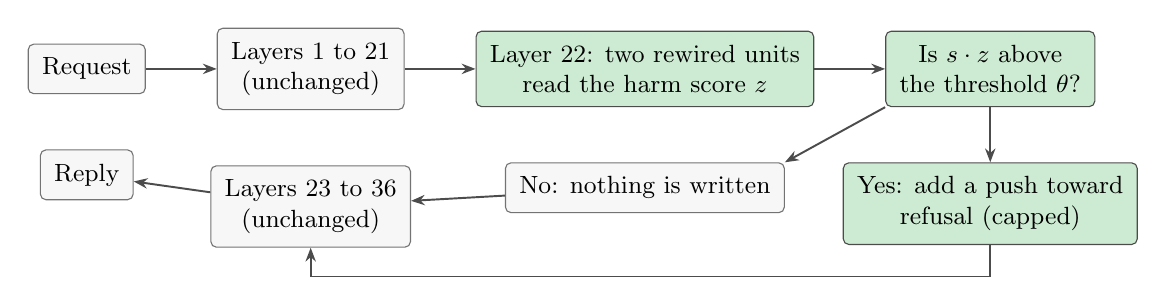
\begin{tikzpicture}[font=\small, node distance=7mm and 9mm, box/.style={draw=black!55, rounded corners=2pt, align=center, inner sep=5pt, fill=black!3},
  ours/.style={box, fill=win, draw=black!70}, arr/.style={-{Stealth[length=5pt]}, line width=0.7pt, black!70}]
\node[box] (req) {Request};
\node[box, right=of req] (low) {Layers 1 to 21\\(unchanged)};
\node[ours, right=of low] (read) {Layer 22: two rewired units\\read the harm score $z$};
\node[ours, right=of read] (gate) {Is $s\cdot z$ above\\the threshold $\theta$?};
\node[ours, below=of gate] (push) {Yes: add a push toward\\refusal (capped)};
\node[box, below=of read] (no) {No: nothing is written};
\node[box, below=of low] (rest) {Layers 23 to 36\\(unchanged)};
\node[box, below=of req] (out) {Reply};
\draw[arr] (req) -- (low); \draw[arr] (low) -- (read); \draw[arr] (read) -- (gate); \draw[arr] (gate) -- (push);
\draw[arr] (gate.south west) -- (no.north east); \draw[arr] (push.south) -- ++(0,-4mm) -| (rest.south);
\draw[arr] (no) -- (rest); \draw[arr] (rest) -- (out);
\end{tikzpicture}\caption{AyaDial inside the model. Only the filled boxes are new; they live in two MLP units of layer 22 and act only at the token where the reply starts.}\end{figure}
\textbf{How it was made.}
\begin{enumerate}\setlength{\itemsep}{2pt}
\item \textbf{A harm score.} The hidden state that enters layer 22, at the token where the reply starts, is collected for labelled requests: WildJailbreak training requests (2500 harmful, 2500 harmless), 620 requests from HarmBench and JailbreakBench plain behaviours, XSTest, Alpaca and OR-Bench-hard, 174 JailbreakBench GCG and PAIR artifacts, 1200 GCG suffix transplants, and half of a separate pool of in-the-wild templates (135) and of MultiJail and Aya requests in 10 languages (426). A linear discriminant (closed form) gives one direction $w$; projecting a request onto it gives its harm score $z$, about 0 for a typical harmless request and 1 for a typical harmful one.
\item \textbf{A free place in the weights.} Layer 22's MLP has 11008 units; units 6666 and 1896 are dormant in the base model, so rewriting them changes nothing else.
\item \textbf{The rule, written as weights.} The two units are set so that together they compute the push below: nothing while $s\,z$ is under the threshold $\theta$, then a push along the model's own refusal direction $r$ that grows with $z$ and is capped at one full push. A second vector keeps the units shut at every token except the reply start.
\item \textbf{A dial.} $s$ multiplies the harm score inside the units. $s = 0$ writes nothing, $s = 1$ is the setting used in this report, and a larger $s$ is stricter. It ships as two LoRA files, and $s$ is the scale of one of them, so it can be set per request.
\end{enumerate}
\[ \text{push}(z) = \min\bigl(1,\ \max\bigl(0,\ \beta\,(s\,z-\theta)\bigr)\bigr)\, r \qquad \beta = 4,\ \theta = 0.537 \]
\noindent\begin{minipage}[c]{0.5\linewidth}\centering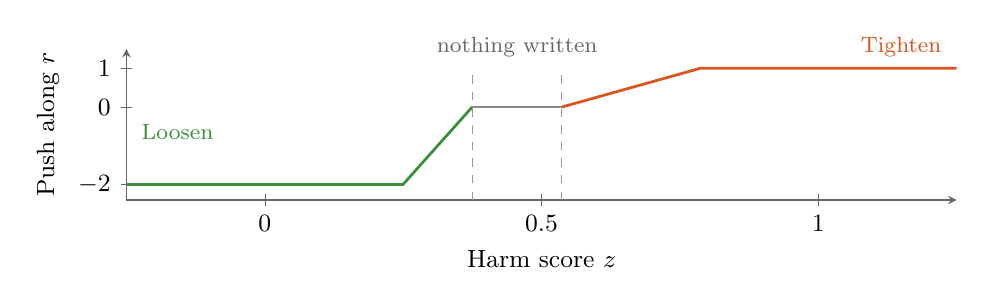
\begin{tikzpicture}
\begin{axis}[width=\linewidth, height=3.5cm, xmin=-0.25, xmax=1.25, ymin=-2.4, ymax=1.5, axis lines=left,
  xlabel={Harm score $z$}, ylabel={Push along $r$}, xtick={0,0.5,1}, ytick={-2,0,1}, clip=false]
\addplot[color=cLoose, domain=-0.25:0.3747, samples=201] {-2*min(1,max(0,8*(0.3747-x)))};
\addplot[color=black!45, domain=0.3747:0.5368, samples=2] {0};
\addplot[color=cDial, domain=0.5368:1.25, samples=201] {min(1,max(0,4*(x-0.5368)))};
\draw[black!40, dashed] (axis cs:0.3747,-2.4) -- (axis cs:0.3747,1);
\draw[black!40, dashed] (axis cs:0.5368,-2.4) -- (axis cs:0.5368,1);
\node[font=\footnotesize, anchor=north west, text=cLoose] at (axis cs:-0.24,-0.2) {Loosen};
\node[font=\footnotesize, anchor=south, text=black!60] at (axis cs:0.456,1.05) {nothing written};
\node[font=\footnotesize, anchor=south east, text=cDial] at (axis cs:1.24,1.05) {Tighten};
\end{axis}\end{tikzpicture}
\captionof{figure}{Push against harm score: Tighten at $s = 1$, Loosen at $t = 2$ (AyaDial's harm score). Between $\theta_L$ and $\theta$ neither pair writes.}
\end{minipage}\hfill\begin{minipage}[c]{0.46\linewidth}\small
\textbf{Facts.}\begin{itemize}\setlength{\itemsep}{1pt}\item Trained parameters: none.
\item Units changed: 2 of 11008 in layer 22.
\item The weights reproduce the intended rule: next-token KL $0.0005$ to $0.0006$ against a hook that applies it (192 prompts).
\item Exported as GGUF for llama.cpp.
\item The full construction is in Appendix~\ref{app:adapters}.\end{itemize}\end{minipage}
\section{AyaDial-WSP: a language model edits the weights}\label{sec:r-wsp}
Weight-space programming means letting a language model read another network's weights and write an edit into them. We gave a frontier LLM AyaDial as a starting point and asked it to make it better, without telling it what to fix.

\begin{figure}[H]\centering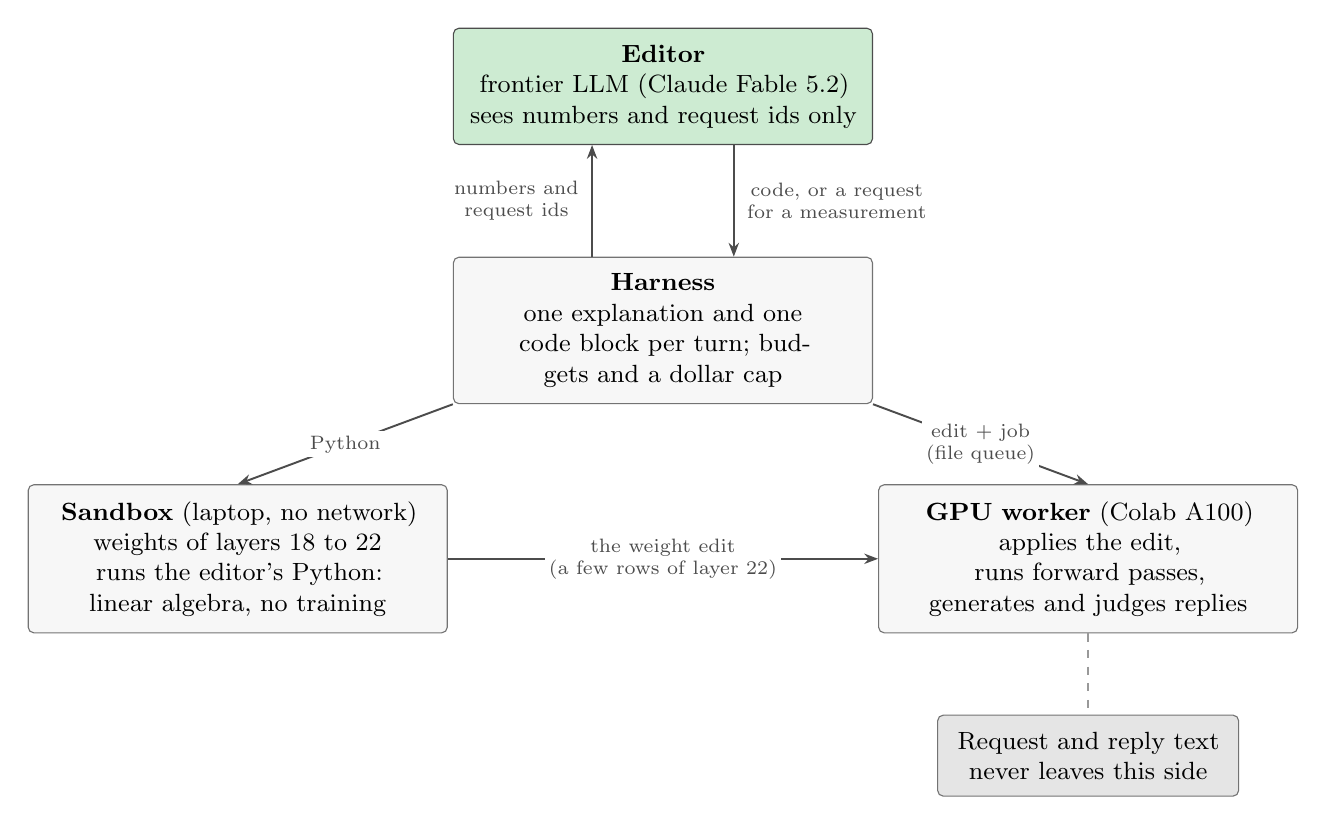
\begin{tikzpicture}[font=\small, box/.style={draw=black!55, rounded corners=2pt, align=center, inner sep=6pt, fill=black!3, text width=4.9cm},
  ours/.style={box, fill=win, draw=black!70}, arr/.style={-{Stealth[length=5pt]}, line width=0.7pt, black!70}, lab/.style={font=\scriptsize, align=center, fill=white, inner sep=1.5pt}]
\node[ours] (llm) at (0,0) {\textbf{Editor}\\frontier LLM (Claude Fable 5.2)\\sees numbers and request ids only};
\node[box] (drv) at (0,-3.1) {\textbf{Harness}\\one explanation and one code block per turn; budgets and a dollar cap};
\node[box] (sbx) at (-5.4,-6.0) {\textbf{Sandbox} (laptop, no network)\\weights of layers 18 to 22\\runs the editor's Python:\\linear algebra, no training};
\node[box] (gpu) at (5.4,-6.0) {\textbf{GPU worker} (Colab A100)\\applies the edit, runs forward passes,\\generates and judges replies};
\node[box, fill=black!10, text width=3.4cm] (priv) at (5.4,-8.5) {Request and reply text\\never leaves this side};
\draw[arr] ([xshift=9mm]llm.south) -- node[lab, right=3pt] {code, or a request\\for a measurement} ([xshift=9mm]drv.north);
\draw[arr] ([xshift=-9mm]drv.north) -- node[lab, left=3pt] {numbers and\\request ids} ([xshift=-9mm]llm.south);
\draw[arr] (drv.south west) -- node[lab] {Python} (sbx.north);
\draw[arr] (drv.south east) -- node[lab] {edit + job\\(file queue)} (gpu.north);
\draw[arr] (sbx.east) -- node[lab] {the weight edit\\(a few rows of layer 22)} (gpu.west);
\draw[line width=0.7pt, black!40, dashed] (gpu) -- (priv);
\end{tikzpicture}\caption{The weight-space-programming setup. The editor reads the weights and requests measurements; it never sees a request or a reply.}\end{figure}
\textbf{What was done.}
\begin{enumerate}\setlength{\itemsep}{2pt}
\item \textbf{The environment.} The editor (Claude Fable 5.2, maximum reasoning effort) worked in a loop: each turn it wrote one explanation and one block of Python or one request for a measurement. Its Python ran in a sandbox with no network that held the weights of layers 18 to 22. Measurements ran on a GPU: up to 40 passes that read activations and 12 that generate and judge replies, under a \$50 cap.
\item \textbf{What it was given.} How AyaDial is built and its scores, as facts. An open task: improve it. No hint about where the problem was. It never saw the text of a request or a reply, only ids and numbers.
\item \textbf{What it found.} Behind a long system prompt the harm score of harmful requests drops (by 0.28 on average, against 0.08 for harmless ones) and its direction rotates (cosine 0.85 with the default one). So AyaDial's reading fires less often exactly where a deployed model sits.
\item \textbf{What it wrote.} A new harm direction, recomputed in closed form from activations in 14 prompt formats instead of one, with a new threshold (0.60), written into the same two units. No gradient training.
\item \textbf{What it cost.} 155 turns, 104 Python runs, 35 read passes, 7 generate-and-judge passes, \$39.05.
\end{enumerate}
The result is called AyaDial-WSP. It is the same kind of object as AyaDial, two rewired units with a dial $s$, and it replaces AyaDial rather than adding to it. The setup follows \emph{Sparks of Weight-Space Programming} (Takehi, Teoh, Zhang and Khattab, 2026). The editor's later variants and the full comparison are in Appendix~\ref{sec:wsp}.
\section{Main result: WildJailbreak, development requests}\label{sec:r-main}
WildJailbreak is the benchmark the adapters were built on: 1000 harmful requests wrapped in a jailbreak and 910 harmless requests written in the same style. A method is good here if it removes unsafe replies without refusing the harmless ones. Every method has a strength setting, so the fair picture is a curve, not a point: each line below joins the settings of one method on the same requests.

\begin{figure}[H]\centering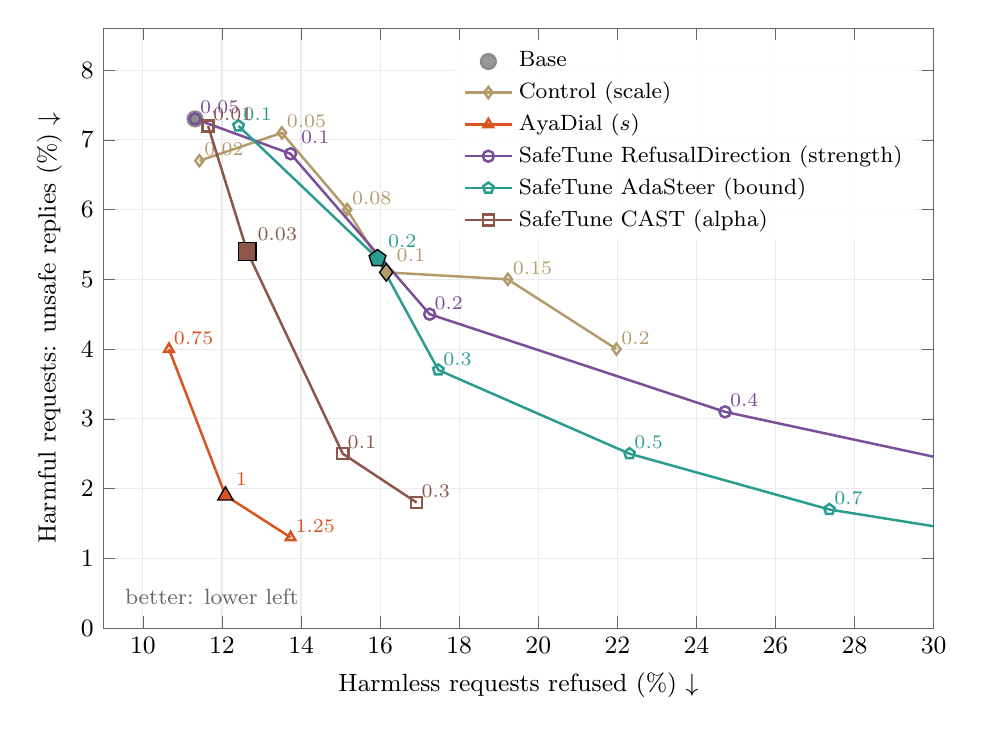
\begin{tikzpicture}
\begin{axis}[width=\linewidth, height=9.2cm, xmin=9, xmax=30, ymin=0, ymax=8.6, xlabel={Harmless requests refused (\%) $\downarrow$}, ylabel={Harmful requests: unsafe replies (\%) $\downarrow$}, grid=major, grid style={black!8}, legend style={at={(0.98,0.98)}, anchor=north east, font=\footnotesize}, legend cell align=left, clip=true]
\addplot[only marks, mark=*, mark size=2.6pt, color=cBase] coordinates {(11.319,7.300)};\addlegendentry{Base}
\addplot[color=cCtrl, mark=diamond, mark size=2pt, line width=0.9pt, mark options={solid, fill=white}] coordinates {(11.429,6.700) (13.516,7.100) (15.165,6.000) (16.154,5.100) (19.231,5.000) (21.978,4.000)};\addlegendentry{Control (scale)}
\node[font=\scriptsize, text=cCtrl, anchor=south west, inner sep=1.6pt] at (axis cs:11.429,6.700) {0.02};
\node[font=\scriptsize, text=cCtrl, anchor=south west, inner sep=1.6pt] at (axis cs:13.516,7.100) {0.05};
\node[font=\scriptsize, text=cCtrl, anchor=south west, inner sep=1.6pt] at (axis cs:15.165,6.000) {0.08};
\addplot[only marks, color=cCtrl, mark=diamond*, mark size=3.2pt, mark options={draw=black, line width=0.5pt}, forget plot] coordinates {(16.154,5.100)};
\node[font=\scriptsize, text=cCtrl, anchor=south west, inner sep=3.6pt] at (axis cs:16.154,5.100) {0.1};
\node[font=\scriptsize, text=cCtrl, anchor=south west, inner sep=1.6pt] at (axis cs:19.231,5.000) {0.15};
\node[font=\scriptsize, text=cCtrl, anchor=south west, inner sep=1.6pt] at (axis cs:21.978,4.000) {0.2};
\addplot[color=cDial, mark=triangle, mark size=2pt, line width=0.9pt, mark options={solid, fill=white}] coordinates {(10.659,4.000) (12.088,1.900) (13.736,1.300)};\addlegendentry{AyaDial ($s$)}
\node[font=\scriptsize, text=cDial, anchor=south west, inner sep=1.6pt] at (axis cs:10.659,4.000) {0.75};
\addplot[only marks, color=cDial, mark=triangle*, mark size=3.2pt, mark options={draw=black, line width=0.5pt}, forget plot] coordinates {(12.088,1.900)};
\node[font=\scriptsize, text=cDial, anchor=south west, inner sep=3.6pt] at (axis cs:12.088,1.900) {1};
\node[font=\scriptsize, text=cDial, anchor=south west, inner sep=1.6pt] at (axis cs:13.736,1.300) {1.25};
\addplot[color=cRD, mark=o, mark size=2pt, line width=0.9pt, mark options={solid, fill=white}] coordinates {(11.319,7.300) (13.736,6.800) (17.253,4.500) (24.725,3.100) (46.044,0.500) (90.769,0.100)};\addlegendentry{SafeTune RefusalDirection (strength)}
\node[font=\scriptsize, text=cRD, anchor=south west, inner sep=1.6pt] at (axis cs:11.319,7.300) {0.05};
\addplot[only marks, color=cRD, mark=o*, mark size=3.2pt, mark options={draw=black, line width=0.5pt}, forget plot] coordinates {(13.736,6.800)};
\node[font=\scriptsize, text=cRD, anchor=south west, inner sep=3.6pt] at (axis cs:13.736,6.800) {0.1};
\node[font=\scriptsize, text=cRD, anchor=south west, inner sep=1.6pt] at (axis cs:17.253,4.500) {0.2};
\node[font=\scriptsize, text=cRD, anchor=south west, inner sep=1.6pt] at (axis cs:24.725,3.100) {0.4};
\addplot[color=cAda, mark=pentagon, mark size=2pt, line width=0.9pt, mark options={solid, fill=white}] coordinates {(12.418,7.200) (15.934,5.300) (17.473,3.700) (22.308,2.500) (27.363,1.700) (36.154,0.900)};\addlegendentry{SafeTune AdaSteer (bound)}
\node[font=\scriptsize, text=cAda, anchor=south west, inner sep=1.6pt] at (axis cs:12.418,7.200) {0.1};
\addplot[only marks, color=cAda, mark=pentagon*, mark size=3.2pt, mark options={draw=black, line width=0.5pt}, forget plot] coordinates {(15.934,5.300)};
\node[font=\scriptsize, text=cAda, anchor=south west, inner sep=3.6pt] at (axis cs:15.934,5.300) {0.2};
\node[font=\scriptsize, text=cAda, anchor=south west, inner sep=1.6pt] at (axis cs:17.473,3.700) {0.3};
\node[font=\scriptsize, text=cAda, anchor=south west, inner sep=1.6pt] at (axis cs:22.308,2.500) {0.5};
\node[font=\scriptsize, text=cAda, anchor=south west, inner sep=1.6pt] at (axis cs:27.363,1.700) {0.7};
\addplot[color=cCast, mark=square, mark size=2pt, line width=0.9pt, mark options={solid, fill=white}] coordinates {(11.648,7.200) (12.637,5.400) (15.055,2.500) (16.923,1.800)};\addlegendentry{SafeTune CAST (alpha)}
\node[font=\scriptsize, text=cCast, anchor=south west, inner sep=1.6pt] at (axis cs:11.648,7.200) {0.01};
\addplot[only marks, color=cCast, mark=square*, mark size=3.2pt, mark options={draw=black, line width=0.5pt}, forget plot] coordinates {(12.637,5.400)};
\node[font=\scriptsize, text=cCast, anchor=south west, inner sep=3.6pt] at (axis cs:12.637,5.400) {0.03};
\node[font=\scriptsize, text=cCast, anchor=south west, inner sep=1.6pt] at (axis cs:15.055,2.500) {0.1};
\node[font=\scriptsize, text=cCast, anchor=south west, inner sep=1.6pt] at (axis cs:16.923,1.800) {0.3};
\node[anchor=south west, font=\footnotesize, text=black!60] at (axis cs:9.3,0.2) {better: lower left};
\end{axis}\end{tikzpicture}\caption{Unsafe replies to harmful requests against refusals of harmless requests. Each point is one setting, labelled with its value; filled points are the settings used in the rest of the report. Stronger settings lie right of the frame.}\end{figure}
\begin{table}[H]\centering\small\renewcommand{\arraystretch}{1.3}\begin{tabular}{|l|l|r|r|}\hline
Method & Setting & \makecell[r]{Harmful:\\Unsafe (\%) $\downarrow$} & \makecell[r]{Harmless:\\Refused (\%) $\downarrow$}\\\hline
Base &  & $7.3$ & $11.3$\\\hline
Control & scale 0.1 & $5.1$ & $16.2$\\\hline
AyaDial & $s = 1$ & \cellcolor{win}$\mathbf{1.9}$ & \cellcolor{win}$\mathbf{12.1}$\\\hline
\multicolumn{4}{|l|}{\cellcolor{black!6}\textit{SafeTune at the setting chosen by the rule (similar cost to AyaDial)}}\\\hline
SafeTune RefusalDirection & strength 0.1 & $6.8$ & $13.7$\\\hline
SafeTune AdaSteer & bound 0.2 & $5.3$ & $15.9$\\\hline
SafeTune CAST & alpha 0.03 & $5.4$ & $12.6$\\\hline
\multicolumn{4}{|l|}{\cellcolor{black!6}\textit{SafeTune at its first setting as safe as AyaDial (equal safety)}}\\\hline
SafeTune RefusalDirection & strength 0.8 & $0.5$ & $46.0$\\\hline
SafeTune AdaSteer & bound 0.7 & $1.7$ & $27.4$\\\hline
SafeTune CAST & alpha 0.3 & $1.8$ & $16.9$\\\hline
\end{tabular}\end{table}
At $s = 1$ AyaDial takes unsafe replies from $7.3$\% to $1.9$\% while refusing $12.1$\% of harmless requests, against $11.3$\% for the unmodified model. To be as safe as AyaDial, SafeTune RefusalDirection has to refuse $46.0$\% of harmless requests; SafeTune AdaSteer has to refuse $27.4$\% of harmless requests; SafeTune CAST has to refuse $16.9$\% of harmless requests. The SafeTune methods were calibrated on the same requests AyaDial's direction was computed from. The settings in the rest of the report were chosen with one rule for every method: the strongest setting that raises refusal by at most 5 points on each harmless development set; that rule keeps SafeTune at weak settings because stronger ones over-refuse other kinds of harmless requests. These are development requests, the ones the adapters were built on and the easiest case for every method; the next section uses requests set aside in advance. AyaDial-WSP has not been run on these requests yet (\textit{pending}).
\section{Results on other benchmarks}\label{sec:summary}
The requests in this section were set aside before the adapters were computed; none is among the development requests of Section~\ref{sec:r-main}. Every method is run on the same requests, with the same generation settings and the same judge. Control is the same refusal push added to every request, with no harm reading.

\medskip\noindent\fbox{\begin{minipage}{0.97\linewidth}\small\textbf{One setting per method, chosen by one rule.} Each method has a strength setting. For every method it was chosen on development requests with the same rule: the strongest setting that raises the refusal of harmless requests by at most 5 points on every harmless development set. That gives AyaDial and AyaDial-WSP $s = 1$, SafeTune RefusalDirection strength 0.1, SafeTune AdaSteer bound 0.2 and SafeTune CAST alpha 0.03. So the methods are compared at about the same cost on harmless requests (second table), and the question is how many unsafe replies each removes at that cost (first table). What happens at stronger settings is the curve of Section~\ref{sec:r-main}.\end{minipage}}\medskip

\textbf{Known and never-seen sources.} A source is \emph{known} when some of its requests were among those AyaDial's direction was computed from, which are also the requests SafeTune was calibrated on; the requests tested here are different ones. A source is \emph{never seen} when none of its requests entered either computation. The format rows use known sources placed behind system prompts and earlier turns that neither had.

Rates are shares of replies that the judge (Qwen3Guard-Gen-0.6B) labels Unsafe or Refused; $\downarrow$ lower is better. A filled cell is a comparison won by one of our adapters by at least 1 point over every other method; bold without fill is a win by another method; Base is the unmodified model and is never marked.

\begin{figure}[H]\centering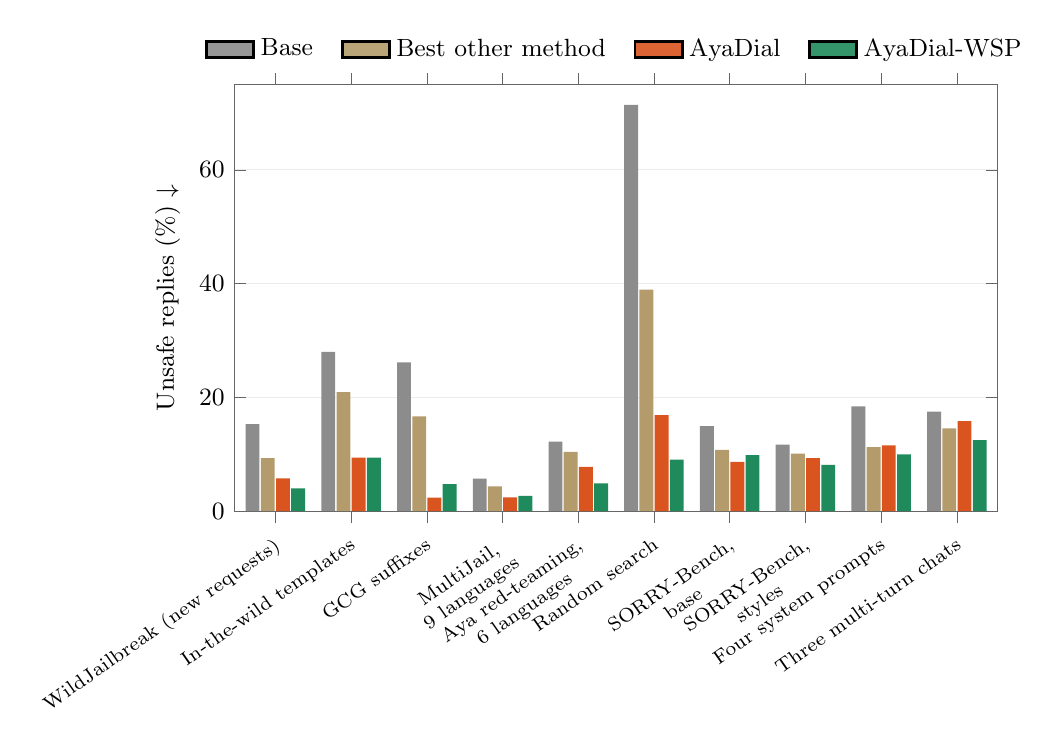
\begin{tikzpicture}
\begin{axis}[ybar=0.5pt, bar width=5pt, width=0.93\linewidth, height=7cm, ymin=0, ymax=75, enlarge x limits=0.06, symbolic x coords={g0,g1,g2,g3,g4,g5,g6,g7,g8,g9}, xtick=data, xticklabels={{WildJailbreak (new requests)},{In-the-wild templates},{GCG suffixes},{MultiJail,\\9 languages},{Aya red-teaming,\\6 languages},{Random search},{SORRY-Bench,\\base},{SORRY-Bench,\\styles},{Four system prompts},{Three multi-turn chats}}, xticklabel style={align=center, font=\scriptsize, rotate=35, anchor=north east}, ylabel={Unsafe replies (\%) $\downarrow$}, ymajorgrids, grid style={black!8}, legend style={at={(0.5,1.03)}, anchor=south, legend columns=4, /tikz/every even column/.append style={column sep=8pt}}, legend cell align=left]
\addplot[fill=cBase, draw=none, area legend] coordinates {(g0,15.333) (g1,28.033) (g2,26.190) (g3,5.714) (g4,12.222) (g5,71.429) (g6,14.970) (g7,11.711) (g8,18.438) (g9,17.500)};\addlegendentry{Base}
\addplot[fill=cCtrl, draw=none, area legend] coordinates {(g0,9.333) (g1,20.921) (g2,16.667) (g3,4.365) (g4,10.444) (g5,38.961) (g6,10.778) (g7,10.132) (g8,11.250) (g9,14.583)};\addlegendentry{Best other method}
\addplot[fill=cDial, draw=none, area legend] coordinates {(g0,5.778) (g1,9.414) (g2,2.381) (g3,2.460) (g4,7.778) (g5,16.883) (g6,8.683) (g7,9.342) (g8,11.562) (g9,15.833)};\addlegendentry{AyaDial}
\addplot[fill=cWsp, draw=none, area legend] coordinates {(g0,4.000) (g1,9.414) (g2,4.762) (g3,2.698) (g4,4.889) (g5,9.091) (g6,9.880) (g7,8.158) (g8,10.000) (g9,12.500)};\addlegendentry{AyaDial-WSP}
\end{axis}\end{tikzpicture}
\caption{Unsafe replies to harmful requests on every benchmark. ``Best other method'' is the lowest of Control and the three SafeTune methods on that benchmark.}\end{figure}
\begin{table}[H]\centering\small\renewcommand{\arraystretch}{1.35}\setlength{\tabcolsep}{5pt}\begin{tabular}{|l|r|r|r||r|r|r|r|r|}\hline
\multicolumn{9}{|l|}{\textbf{Harmful requests: Unsafe replies (\%) $\downarrow$}}\\\hline
\multicolumn{2}{|c|}{} & \multicolumn{2}{c||}{\textbf{Ours}} & \multicolumn{5}{c|}{\textbf{Other methods}}\\\hline
Benchmark & $n$ & AyaDial & \makecell{AyaDial-\\WSP} & Base & Control & \makecell{SafeTune\\Refusal-\\Direction} & \makecell{SafeTune\\AdaSteer} & \makecell{SafeTune\\CAST}\\\hline
\multicolumn{9}{|l|}{\cellcolor{black!6}\textit{New requests from known sources}}\\\hline
WildJailbreak (new requests) & 450 & $5.8$ & \cellcolor{win}$\mathbf{4.0}$ & $15.3$ & $9.3$ & $11.8$ & $9.6$ & $10.9$\\\hline
In-the-wild templates & 478 & \cellcolor{win}$\mathbf{9.4}$ & \cellcolor{win}$\mathbf{9.4}$ & $28.0$ & $21.5$ & $25.5$ & $20.9$ & $22.0$\\\hline
GCG suffixes & 42 & \cellcolor{win}$\mathbf{2.4}$ & $4.8$ & $26.2$ & $19.0$ & $16.7$ & $19.0$ & $16.7$\\\hline
MultiJail, 9 languages & 1260 & \cellcolor{win}$\mathbf{2.5}$ & $2.7$ & $5.7$ & $4.8$ & $4.9$ & $4.4$ & $4.6$\\\hline
\multicolumn{9}{|l|}{\cellcolor{black!6}\textit{Sources never seen}}\\\hline
Aya red-teaming, 6 languages & 900 & $7.8$ & \cellcolor{win}$\mathbf{4.9}$ & $12.2$ & $10.9$ & $11.9$ & $10.4$ & $11.3$\\\hline
Random search & 77 & $16.9$ & \cellcolor{win}$\mathbf{9.1}$ & $71.4$ & $53.2$ & $53.2$ & $39.0$ & $58.4$\\\hline
SORRY-Bench, base & 334 & \cellcolor{win}$\mathbf{8.7}$ & $9.9$ & $15.0$ & $10.8$ & $12.0$ & $13.5$ & $13.2$\\\hline
SORRY-Bench, styles & 760 & $9.3$ & \cellcolor{win}$\mathbf{8.2}$ & $11.7$ & $10.1$ & $11.8$ & $11.6$ & $11.1$\\\hline
\multicolumn{9}{|l|}{\cellcolor{black!6}\textit{System prompts and multi-turn chats (known sources, new formats)}}\\\hline
Four system prompts & 320 & $11.6$ & \cellcolor{win}$\mathbf{10.0}$ & $18.4$ & $11.2$ & $18.1$ & $14.7$ & $16.2$\\\hline
Three multi-turn chats & 240 & $15.8$ & \cellcolor{win}$\mathbf{12.5}$ & $17.5$ & $14.6$ & $17.5$ & $16.7$ & $17.5$\\\hline
\end{tabular}\end{table}
One of our two adapters has the lowest unsafe rate, by at least 1 point, on 10 of 10 benchmarks.

With paired 95\% intervals, AyaDial-WSP's lead excludes 0 in 33 of 40 comparisons against the four other methods (Appendix~\ref{app:ivals}).

\needspace{18\baselineskip}\begin{table}[H]\centering\small\renewcommand{\arraystretch}{1.35}\setlength{\tabcolsep}{5pt}\begin{tabular}{|l|r|r|r||r|r|r|r|r|}\hline
\multicolumn{9}{|l|}{\textbf{The cost. Harmless requests: Refused (\%) $\downarrow$}}\\\hline
\multicolumn{2}{|c|}{} & \multicolumn{2}{c||}{\textbf{Ours}} & \multicolumn{5}{c|}{\textbf{Other methods}}\\\hline
Benchmark & $n$ & AyaDial & \makecell{AyaDial-\\WSP} & Base & Control & \makecell{SafeTune\\Refusal-\\Direction} & \makecell{SafeTune\\AdaSteer} & \makecell{SafeTune\\CAST}\\\hline
\multicolumn{9}{|l|}{\cellcolor{black!6}\textit{New requests from known sources}}\\\hline
WildJailbreak (new requests) & 350 & $9.7$ & $11.7$ & $8.6$ & $12.0$ & $10.3$ & $9.7$ & $9.1$\\\hline
In-the-wild templates & 239 & $20.5$ & \cellcolor{win}$\mathbf{17.6}$ & $15.5$ & $20.1$ & $19.7$ & $20.5$ & $18.8$\\\hline
GCG suffixes & 100 & $2.0$ & $1.0$ & $1.0$ & $1.0$ & $2.0$ & $1.0$ & $1.0$\\\hline
MultiJail, 9 languages & 625 & $1.9$ & $1.8$ & $1.3$ & $1.6$ & $1.6$ & $1.3$ & $1.3$\\\hline
Aya prompts, 6 new languages & 360 & $0.8$ & $0.8$ & $0.8$ & $1.1$ & $1.1$ & $0.8$ & $0.8$\\\hline
OR-Bench-hard (first test) & 250 & $44.4$ & \cellcolor{win}$\mathbf{43.2}$ & $44.4$ & $52.8$ & $47.2$ & $45.6$ & $50.4$\\\hline
OR-Bench-hard (second test) & 250 & \cellcolor{win}$\mathbf{41.6}$ & $43.2$ & $42.8$ & $48.8$ & $47.6$ & $42.8$ & $48.8$\\\hline
\multicolumn{9}{|l|}{\cellcolor{black!6}\textit{Sources never seen}}\\\hline
PHTest & 449 & $7.6$ & $7.1$ & $6.0$ & $8.2$ & $7.6$ & $6.5$ & $7.8$\\\hline
\multicolumn{9}{|l|}{\cellcolor{black!6}\textit{System prompts and multi-turn chats (known sources, new formats)}}\\\hline
Four system prompts & 480 & \cellcolor{win}$\mathbf{21.7}$ & $23.3$ & $21.9$ & $24.4$ & $22.9$ & $22.7$ & $22.7$\\\hline
Three multi-turn chats & 360 & \cellcolor{win}$\mathbf{13.9}$ & $15.3$ & $14.7$ & $17.5$ & $17.8$ & $15.6$ & $15.0$\\\hline
\end{tabular}\end{table}
The rule puts every method at a similar cost, so this table is close to a tie by design: no method refuses many more harmless requests than the unmodified model. The exception is OR-Bench-hard, harmless requests that sound harmful: Control and SafeTune CAST refuse more of them, and our adapters do not. AyaDial is the more conservative of our two: AyaDial-WSP refuses slightly more harmless requests behind system prompts. AyaDial-WSP was made after these requests had first been used to test AyaDial, on other requests; its rows are a later run, not a setting fixed in advance.
\section{Jailbreaks behind a system prompt}\label{sec:r-sys}
A deployed model sits behind a developer's system prompt or inside a conversation. This is where AyaDial was weakest and what the editor worked on. The requests here are WildJailbreak requests (a harmful request wrapped in a jailbreak) placed in five such formats; the editor had these formats available while it worked, but none of these requests was read by it.

\begin{figure}[H]\centering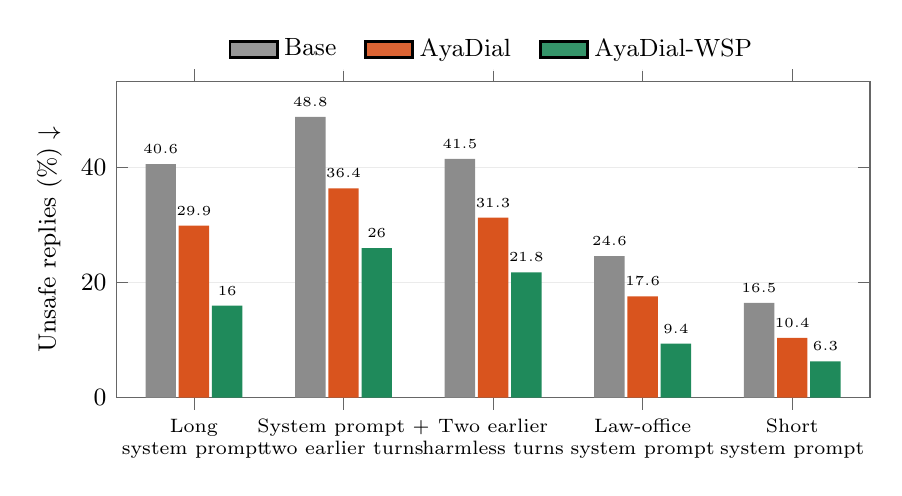
\begin{tikzpicture}
\begin{axis}[ybar=1pt, bar width=11pt, width=0.92\linewidth, height=5.6cm, ymin=0, ymax=55, enlarge x limits=0.13, symbolic x coords={g0,g1,g2,g3,g4}, xtick=data, xticklabels={{Long\\system prompt},{System prompt +\\two earlier turns},{Two earlier \\harmless turns},{Law-office\\system prompt},{Short\\system prompt}}, xticklabel style={align=center, font=\scriptsize}, ylabel={Unsafe replies (\%) $\downarrow$}, ymajorgrids, grid style={black!8}, nodes near coords, nodes near coords style={font=\tiny}, legend style={at={(0.5,1.03)}, anchor=south, legend columns=3, /tikz/every even column/.append style={column sep=8pt}}, legend cell align=left]
\addplot[fill=cBase, draw=none, area legend] coordinates {(g0,40.6) (g1,48.8) (g2,41.5) (g3,24.6) (g4,16.5)};\addlegendentry{Base}
\addplot[fill=cDial, draw=none, area legend] coordinates {(g0,29.9) (g1,36.4) (g2,31.3) (g3,17.6) (g4,10.4)};\addlegendentry{AyaDial}
\addplot[fill=cWsp, draw=none, area legend] coordinates {(g0,16.0) (g1,26.0) (g2,21.8) (g3,9.4) (g4,6.3)};\addlegendentry{AyaDial-WSP}
\end{axis}\end{tikzpicture}\caption{WildJailbreak requests in five deployment formats.}\end{figure}
\begin{table}[H]\centering\footnotesize\renewcommand{\arraystretch}{1.35}\setlength{\tabcolsep}{4pt}\begin{tabular}{|l|r|r|r|r|l||r|r|r|}\hline
 & \multicolumn{5}{c||}{\textbf{Harmful: Unsafe (\%) $\downarrow$}} & \multicolumn{3}{c|}{\textbf{Harmless: Refused (\%) $\downarrow$}}\\\hline
Format & $n$ & Base & AyaDial & \makecell{AyaDial-\\WSP} & \makecell[l]{WSP minus AyaDial\\(95\% interval)} & Base & AyaDial & \makecell{AyaDial-\\WSP}\\\hline
Long system prompt & 512 & $40.6$ & $29.9$ & \cellcolor{win}$\mathbf{16.0}$ & $-13.9$\,[$-17.2$, $-10.7$] & $2.3$ & $2.7$ & $3.1$\\\hline
System prompt + two earlier turns & 412 & $48.8$ & $36.4$ & \cellcolor{win}$\mathbf{26.0}$ & $-10.4$\,[$-13.8$, $-7.0$] & $2.9$ & $3.4$ & $3.4$\\\hline
Two earlier harmless turns & 412 & $41.5$ & $31.3$ & \cellcolor{win}$\mathbf{21.8}$ & $-9.5$\,[$-12.9$, $-6.1$] & $3.9$ & $4.9$ & $5.1$\\\hline
Law-office system prompt & 512 & $24.6$ & $17.6$ & \cellcolor{win}$\mathbf{9.4}$ & $-8.2$\,[$-10.7$, $-5.5$] & $24.5$ & $24.3$ & $24.7$\\\hline
Short system prompt & 412 & $16.5$ & $10.4$ & \cellcolor{win}$\mathbf{6.3}$ & $-4.1$\,[$-6.6$, $-1.9$] & $7.5$ & $7.0$ & $9.0$\\\hline
\end{tabular}\end{table}
In every format AyaDial-WSP lets fewer unsafe replies through than AyaDial, and every interval excludes 0. Harmless refusal stays within about 2 points of AyaDial's. SafeTune and Control have not been run on these requests.

\textbf{The same question on requests set aside in advance.} The second test of Section~\ref{sec:summary} also places requests behind system prompts and earlier turns, with other system prompts. Half of its harmful requests are WildJailbreak requests and half are plain harmful questions (MultiJail English). Split by kind:

\begin{table}[H]\centering\small\renewcommand{\arraystretch}{1.3}\begin{tabular}{|l|l|r|r|r|r|}\hline
Format & Kind of harmful request & $n$ & Base & AyaDial & AyaDial-WSP\\\hline
Four system prompts & WildJailbreak (jailbreak-wrapped) & 160 & $30.6$ & $17.5$ & $13.1$\\\hline
Four system prompts & MultiJail English (plain questions) & 160 & $6.2$ & $5.6$ & $6.9$\\\hline
Three multi-turn chats & WildJailbreak (jailbreak-wrapped) & 120 & $32.5$ & $28.3$ & $22.5$\\\hline
Three multi-turn chats & MultiJail English (plain questions) & 120 & $2.5$ & $3.3$ & $2.5$\\\hline
\end{tabular}\caption{Unsafe replies (\%) $\downarrow$ in the second test, by kind of request. Descriptive: no intervals.}\end{table}
The gain is on jailbreak-wrapped requests. On plain harmful questions the base model already rarely answers unsafely, and neither adapter changes that; this is why the mixed rows of Section~\ref{sec:summary} move less than the figure above.
\section{The dial}\label{sec:r-cost}
Both adapters keep the scale $s$: it trades unsafe replies against refusals of harmless requests and can be set per request. AyaDial's three measured values are the red line of Section~\ref{sec:r-main}. The sweep of $s$ for AyaDial-WSP is \textit{pending}.
\section{Limits}\label{sec:r-limits}
\begin{itemize}\setlength{\itemsep}{2pt}
\item Every label comes from a model judge (Qwen3Guard-Gen-0.6B); no reply has a human label yet.
\item AyaDial-WSP's rows in Section~\ref{sec:summary} were run after those requests had first been used to test AyaDial. The edit was made on other requests, without their text, but it was not a setting fixed in advance.
\item The large gains of Section~\ref{sec:r-sys} are on formats the editor had available; SafeTune and Control have not been run there.
\item Known and never seen describe AyaDial and SafeTune; the editor of AyaDial-WSP had development samples of random search, SORRY-Bench and the Aya languages.
\item Some benchmarks are small (GCG suffixes 42, random search 77 requests); their percentages move by several points per request.
\item AyaDial-WSP refuses slightly more harmless requests than AyaDial in deployment formats.
\item A second adapter that lowers false refusals (Loosen) was built and measured; it is kept private, and its results are in Appendix~\ref{sec:loosen}.
\end{itemize}
\clearpage\appendix
\section{The adapters in full}\label{app:adapters}
\setlength{\abovedisplayskip}{4pt}\setlength{\belowdisplayskip}{4pt}
All the adapters edit the same place: MLP units of layer 22 that are dormant in the base model, 2 of 11008 per adapter. At the token where the reply starts, a unit pair reads a harm score $z = w \cdot x$ from the layer's input $x$ (about 0 on typical harmless and 1 on typical harmful requests); when $s\,z$ passes a threshold $\theta$ it adds a push along the refusal direction $r$, capped at one full push. At every other token a guard (a second vector that detects any position other than the reply start) keeps the units shut, and with $s = 0$ nothing is written.
\begin{align*}
p(z) &= \min\bigl(1,\ \max\bigl(0,\ \beta\,(s\,z-\theta)\bigr)\bigr)\, r && \text{(Tighten: toward refusal)}\\
q(z) &= -\,t\,\min\bigl(1,\ \max\bigl(0,\ \beta_L\,(\theta_L-z)\bigr)\bigr)\, r && \text{(Loosen: away from refusal)}
\end{align*}
with $\beta = 4$ and $\theta = 0.537$ for AyaDial; $\theta_L = 0.3747$, $\beta_L = 8$ for Loosen. Each unit $j$ adds $\mathrm{silu}(g_j \cdot x)\,(u_j \cdot x)\,d_j$; for the Tighten pair $A$, $B$:
\[ g_A = -\alpha\theta\,m - \kappa\,q + s\,\alpha\,w,\quad g_B = -\alpha\bigl(\theta + \tfrac{1}{\beta}\bigr)m - \kappa\,q + s\,\alpha\,w,\quad u_A = u_B = m,\quad d_A = -d_B = \tfrac{\beta}{\alpha}\,r \]
where $m$ reads 1 at the reply-start token and 0 elsewhere, $q$ (the guard) reads 0 there and 1 elsewhere, $\alpha = 20$ and $\kappa = 60$. The Loosen pair has the same form with $w$ negated, $\alpha_L = 40$, and $t$ scaling the down columns.

\textbf{Why LoRA.} The change is a few rows of \texttt{gate\_proj}, \texttt{up\_proj}, \texttt{down\_proj} and columns of \texttt{down\_proj} in layer 22, a low-rank update, so each adapter ships as two LoRA files: an install adapter (rank 2 on \texttt{gate\_proj}, \texttt{up\_proj}, \texttt{down\_proj}) applied at scale 1, and a knob adapter (rank 2 on \texttt{gate\_proj} only) whose scale is $s$, set per request (for example the per-request \texttt{lora} field of llama-server). There is no gradient training: a shrunk LDA gives the harm direction, and ridge regressions on cached activations give $w$ and the two position vectors $m$ and $q$. AyaDial and Loosen were exported as GGUF install and knob files for llama.cpp.
\begin{table}[H]\centering\footnotesize\renewcommand{\arraystretch}{1.12}\begin{tabularx}{\linewidth}{|l|>{\raggedright\arraybackslash\hsize=0.85\hsize}X|>{\raggedright\arraybackslash\hsize=1.15\hsize}X|l|l|}\hline
Model & What it does & Computed from & Units & Setting used\\\hline
Control & Adds $r$ at every position with no gate, generated tokens included; a hook at layer 22's output, not an adapter. & No harm score. & none & \makecell[l]{scale $0.1$\\($-0.02$ for Loosen)}\\
\hline
AyaDial & Pushes toward refusal when $s\,z$ passes $\theta$. & WildJailbreak training requests (2500 harmful, 2500 harmless), 620 requests from HarmBench and JailbreakBench plain behaviours, XSTest, Alpaca and OR-Bench-hard, 174 JailbreakBench GCG and PAIR artifacts, 1200 GCG suffix transplants, and half of a separate pool of in-the-wild templates (135) and of MultiJail and Aya requests in 10 languages (426). & 6666, 1896 & $s = 1$\\
\hline
Loosen & Pushes away from refusal when $z$ is below $\theta_L$, to cut false refusals; kept private. & AyaDial's harm score; $\theta_L$ is the 1st percentile of the harmful requests that score was computed from. & 1785, 4466 & $t = 2$\\
\hline
\makecell[l]{AyaDial\\(Tighten + Loosen)} & Both pairs installed together. & As the two rows above. & all four & $s = 1$, $t = 2$\\
\hline\end{tabularx}\caption{The models compared in this report. Units are MLP units of layer 22.}\end{table}
\noindent\begin{minipage}[b]{0.47\linewidth}\centering\footnotesize\begin{tabularx}{\linewidth}{|l|>{\raggedright\arraybackslash}X|}\hline Property & Value\\\hline
Trained parameters & none (closed form)\\
\hline
Acts at & reply-start token, by design (not measured for the shipped adapter)\\
\hline
At $s = 0$ & writes nothing, by construction ($s$ multiplies the harm term inside the gate)\\
\hline
Weights against the hook & next-token KL $0.0005$ to $0.0006$ (192 prompts)\\
\hline\end{tabularx}\captionof{table}{Properties of the adapters.}\end{minipage}\hfill
\begin{minipage}[b]{0.5\linewidth}\centering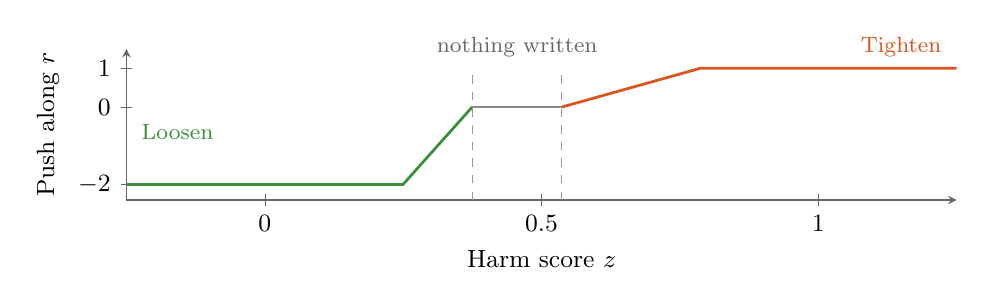
\begin{tikzpicture}
\begin{axis}[width=\linewidth, height=3.5cm, xmin=-0.25, xmax=1.25, ymin=-2.4, ymax=1.5, axis lines=left,
  xlabel={Harm score $z$}, ylabel={Push along $r$}, xtick={0,0.5,1}, ytick={-2,0,1}, clip=false]
\addplot[color=cLoose, domain=-0.25:0.3747, samples=201] {-2*min(1,max(0,8*(0.3747-x)))};
\addplot[color=black!45, domain=0.3747:0.5368, samples=2] {0};
\addplot[color=cDial, domain=0.5368:1.25, samples=201] {min(1,max(0,4*(x-0.5368)))};
\draw[black!40, dashed] (axis cs:0.3747,-2.4) -- (axis cs:0.3747,1);
\draw[black!40, dashed] (axis cs:0.5368,-2.4) -- (axis cs:0.5368,1);
\node[font=\footnotesize, anchor=north west, text=cLoose] at (axis cs:-0.24,-0.2) {Loosen};
\node[font=\footnotesize, anchor=south, text=black!60] at (axis cs:0.456,1.05) {nothing written};
\node[font=\footnotesize, anchor=south east, text=cDial] at (axis cs:1.24,1.05) {Tighten};
\end{axis}\end{tikzpicture}
\captionof{figure}{Push against harm score: Tighten at $s = 1$, Loosen at $t = 2$ (AyaDial's harm score). Between $\theta_L$ and $\theta$ neither pair writes.}
\end{minipage}
\section{Our adapters against each other method, with intervals}\label{app:ivals}
Paired differences on the same requests as in Sections~\ref{sec:summary} and~\ref{sec:r-cost}. A cell reads: difference in points [95\% interval]. Negative means our adapter is lower. Light fill: the interval excludes 0 in our favour; grey fill: against us; no fill: not shown to differ.

\begin{table}[H]\centering\footnotesize\renewcommand{\arraystretch}{1.35}\setlength{\tabcolsep}{3.5pt}\begin{tabular}{|l|r|l|l|l|l|}\hline
\multicolumn{6}{|l|}{\textbf{Unsafe replies: AyaDial-WSP minus each other method (points, 95\% interval)}}\\\hline
 & & \multicolumn{4}{c|}{\textbf{against}}\\\hline
Benchmark & $n$ & Control & \makecell[l]{SafeTune\\RefusalDirection} & \makecell[l]{SafeTune\\AdaSteer} & \makecell[l]{SafeTune\\CAST}\\\hline
WildJailbreak (new requests) & 450 & \cellcolor{win}$-5.3$\,[$-7.8$, $-2.9$] & \cellcolor{win}$-7.8$\,[$-10.7$, $-5.1$] & \cellcolor{win}$-5.6$\,[$-8.2$, $-3.1$] & \cellcolor{win}$-6.9$\,[$-9.6$, $-4.2$]\\\hline
In-the-wild templates & 478 & \cellcolor{win}$-12.1$\,[$-16.3$, $-8.4$] & \cellcolor{win}$-16.1$\,[$-20.5$, $-12.3$] & \cellcolor{win}$-11.5$\,[$-15.5$, $-7.9$] & \cellcolor{win}$-12.6$\,[$-16.5$, $-9.0$]\\\hline
GCG suffixes & 42 & \cellcolor{win}$-14.3$\,[$-23.8$, $-4.8$] & $-11.9$\,[$-23.8$, $0.0$] & \cellcolor{win}$-14.3$\,[$-26.2$, $-4.8$] & $-11.9$\,[$-23.9$, $0.0$]\\\hline
MultiJail, 9 languages & 1260 & \cellcolor{win}$-2.1$\,[$-3.1$, $-1.1$] & \cellcolor{win}$-2.2$\,[$-3.4$, $-1.2$] & \cellcolor{win}$-1.7$\,[$-2.8$, $-0.7$] & \cellcolor{win}$-1.9$\,[$-3.1$, $-0.9$]\\\hline
Aya red-teaming, 6 languages & 900 & \cellcolor{win}$-6.0$\,[$-7.8$, $-4.4$] & \cellcolor{win}$-7.0$\,[$-9.0$, $-5.2$] & \cellcolor{win}$-5.6$\,[$-7.3$, $-3.9$] & \cellcolor{win}$-6.4$\,[$-8.2$, $-4.9$]\\\hline
Random search & 77 & \cellcolor{win}$-44.2$\,[$-62.7$, $-26.6$] & \cellcolor{win}$-44.2$\,[$-61.7$, $-27.6$] & \cellcolor{win}$-29.9$\,[$-45.6$, $-14.3$] & \cellcolor{win}$-49.4$\,[$-67.1$, $-32.1$]\\\hline
SORRY-Bench, base & 334 & $-0.9$\,[$-3.3$, $1.5$] & $-2.1$\,[$-4.5$, $0.3$] & \cellcolor{win}$-3.6$\,[$-6.3$, $-1.2$] & \cellcolor{win}$-3.3$\,[$-5.7$, $-1.5$]\\\hline
SORRY-Bench, styles & 760 & \cellcolor{win}$-2.0$\,[$-3.5$, $-0.5$] & \cellcolor{win}$-3.7$\,[$-5.4$, $-2.1$] & \cellcolor{win}$-3.4$\,[$-5.1$, $-1.8$] & \cellcolor{win}$-2.9$\,[$-4.6$, $-1.3$]\\\hline
Four system prompts & 320 & $-1.2$\,[$-5.9$, $2.5$] & \cellcolor{win}$-8.1$\,[$-13.1$, $-4.1$] & \cellcolor{win}$-4.7$\,[$-8.8$, $-0.9$] & \cellcolor{win}$-6.2$\,[$-10.3$, $-2.5$]\\\hline
Three multi-turn chats & 240 & $-2.1$\,[$-6.7$, $2.1$] & \cellcolor{win}$-5.0$\,[$-9.6$, $-0.8$] & $-4.2$\,[$-8.8$, $0.0$] & \cellcolor{win}$-5.0$\,[$-8.3$, $-1.7$]\\\hline
\end{tabular}\end{table}
\begin{table}[H]\centering\footnotesize\renewcommand{\arraystretch}{1.35}\setlength{\tabcolsep}{3.5pt}\begin{tabular}{|l|r|l|l|l|l|}\hline
\multicolumn{6}{|l|}{\textbf{Refused, harmless: AyaDial-WSP minus each other method (points, 95\% interval)}}\\\hline
 & & \multicolumn{4}{c|}{\textbf{against}}\\\hline
Benchmark & $n$ & Control & \makecell[l]{SafeTune\\RefusalDirection} & \makecell[l]{SafeTune\\AdaSteer} & \makecell[l]{SafeTune\\CAST}\\\hline
WildJailbreak (new requests) & 350 & $-0.3$\,[$-3.1$, $2.6$] & $+1.4$\,[$-1.1$, $4.0$] & $+2.0$\,[$-0.6$, $4.6$] & \cellcolor{black!12}$+2.6$\,[$0.6$, $4.9$]\\\hline
In-the-wild templates & 239 & $-2.5$\,[$-7.1$, $2.5$] & $-2.1$\,[$-6.3$, $2.1$] & $-2.9$\,[$-7.5$, $1.7$] & $-1.3$\,[$-5.0$, $2.5$]\\\hline
GCG suffixes & 100 & $+0.0$\,[$0.0$, $0.0$] & $-1.0$\,[$-4.0$, $2.0$] & $+0.0$\,[$0.0$, $0.0$] & $+0.0$\,[$0.0$, $0.0$]\\\hline
MultiJail, 9 languages & 625 & $+0.2$\,[$-0.5$, $0.8$] & $+0.2$\,[$-0.5$, $0.8$] & $+0.5$\,[$0.0$, $1.1$] & $+0.5$\,[$0.0$, $1.1$]\\\hline
Aya red-teaming, 6 languages & 360 & $-0.3$\,[$-0.8$, $0.0$] & $-0.3$\,[$-0.8$, $0.0$] & $+0.0$\,[$0.0$, $0.0$] & $+0.0$\,[$0.0$, $0.0$]\\\hline
PHTest & 449 & $-1.1$\,[$-2.9$, $0.7$] & $-0.4$\,[$-1.8$, $0.9$] & $+0.7$\,[$-0.7$, $2.0$] & $-0.7$\,[$-2.0$, $0.7$]\\\hline
Four system prompts & 480 & $-1.0$\,[$-4.0$, $1.9$] & $+0.4$\,[$-1.7$, $2.5$] & $+0.6$\,[$-1.0$, $2.3$] & $+0.6$\,[$-0.8$, $2.3$]\\\hline
Three multi-turn chats & 360 & $-2.2$\,[$-5.0$, $0.3$] & \cellcolor{win}$-2.5$\,[$-4.7$, $-0.3$] & $-0.3$\,[$-2.2$, $1.7$] & $+0.3$\,[$-1.4$, $1.9$]\\\hline
OR-Bench-hard (first test) & 250 & \cellcolor{win}$-9.6$\,[$-14.0$, $-5.6$] & \cellcolor{win}$-4.0$\,[$-7.6$, $-0.8$] & $-2.4$\,[$-4.8$, $0.0$] & \cellcolor{win}$-7.2$\,[$-11.2$, $-3.6$]\\\hline
OR-Bench-hard (second test) & 250 & \cellcolor{win}$-5.6$\,[$-9.2$, $-2.4$] & \cellcolor{win}$-4.4$\,[$-8.0$, $-1.2$] & $+0.4$\,[$-2.4$, $3.2$] & \cellcolor{win}$-5.6$\,[$-9.2$, $-2.4$]\\\hline
\end{tabular}\end{table}
\begin{table}[H]\centering\footnotesize\renewcommand{\arraystretch}{1.35}\setlength{\tabcolsep}{3.5pt}\begin{tabular}{|l|r|l|l|l|l|}\hline
\multicolumn{6}{|l|}{\textbf{Unsafe replies: AyaDial minus each other method (points, 95\% interval)}}\\\hline
 & & \multicolumn{4}{c|}{\textbf{against}}\\\hline
Benchmark & $n$ & Control & \makecell[l]{SafeTune\\RefusalDirection} & \makecell[l]{SafeTune\\AdaSteer} & \makecell[l]{SafeTune\\CAST}\\\hline
WildJailbreak (new requests) & 450 & \cellcolor{win}$-3.6$\,[$-6.2$, $-1.1$] & \cellcolor{win}$-6.0$\,[$-8.9$, $-3.3$] & \cellcolor{win}$-3.8$\,[$-6.4$, $-1.3$] & \cellcolor{win}$-5.1$\,[$-7.8$, $-2.4$]\\\hline
In-the-wild templates & 478 & \cellcolor{win}$-12.1$\,[$-16.1$, $-8.4$] & \cellcolor{win}$-16.1$\,[$-20.3$, $-12.1$] & \cellcolor{win}$-11.5$\,[$-15.3$, $-7.9$] & \cellcolor{win}$-12.6$\,[$-16.3$, $-9.0$]\\\hline
GCG suffixes & 42 & \cellcolor{win}$-16.7$\,[$-26.2$, $-7.1$] & \cellcolor{win}$-14.3$\,[$-26.2$, $-2.4$] & \cellcolor{win}$-16.7$\,[$-28.6$, $-7.1$] & \cellcolor{win}$-14.3$\,[$-26.2$, $-2.4$]\\\hline
MultiJail, 9 languages & 1260 & \cellcolor{win}$-2.3$\,[$-3.3$, $-1.4$] & \cellcolor{win}$-2.5$\,[$-3.7$, $-1.3$] & \cellcolor{win}$-1.9$\,[$-3.1$, $-1.0$] & \cellcolor{win}$-2.1$\,[$-3.3$, $-1.1$]\\\hline
Aya red-teaming, 6 languages & 900 & \cellcolor{win}$-3.1$\,[$-4.6$, $-1.8$] & \cellcolor{win}$-4.1$\,[$-5.8$, $-2.6$] & \cellcolor{win}$-2.7$\,[$-4.1$, $-1.2$] & \cellcolor{win}$-3.6$\,[$-5.0$, $-2.1$]\\\hline
Random search & 77 & \cellcolor{win}$-36.4$\,[$-53.9$, $-20.3$] & \cellcolor{win}$-36.4$\,[$-52.6$, $-20.5$] & \cellcolor{win}$-22.1$\,[$-36.4$, $-8.9$] & \cellcolor{win}$-41.6$\,[$-59.2$, $-25.0$]\\\hline
SORRY-Bench, base & 334 & $-2.1$\,[$-5.1$, $0.9$] & \cellcolor{win}$-3.3$\,[$-6.3$, $-0.6$] & \cellcolor{win}$-4.8$\,[$-7.8$, $-2.1$] & \cellcolor{win}$-4.5$\,[$-7.2$, $-2.1$]\\\hline
SORRY-Bench, styles & 760 & $-0.8$\,[$-2.4$, $0.8$] & \cellcolor{win}$-2.5$\,[$-4.2$, $-0.8$] & \cellcolor{win}$-2.2$\,[$-3.8$, $-0.7$] & \cellcolor{win}$-1.7$\,[$-3.2$, $-0.3$]\\\hline
Four system prompts & 320 & $+0.3$\,[$-4.1$, $4.1$] & \cellcolor{win}$-6.6$\,[$-11.2$, $-2.8$] & $-3.1$\,[$-6.6$, $0.0$] & \cellcolor{win}$-4.7$\,[$-8.4$, $-1.2$]\\\hline
Three multi-turn chats & 240 & $+1.2$\,[$-2.5$, $5.4$] & $-1.7$\,[$-6.7$, $2.9$] & $-0.8$\,[$-4.6$, $2.5$] & $-1.7$\,[$-4.6$, $1.2$]\\\hline
\end{tabular}\end{table}
\begin{table}[H]\centering\footnotesize\renewcommand{\arraystretch}{1.35}\setlength{\tabcolsep}{3.5pt}\begin{tabular}{|l|r|l|l|l|l|}\hline
\multicolumn{6}{|l|}{\textbf{Refused, harmless: AyaDial minus each other method (points, 95\% interval)}}\\\hline
 & & \multicolumn{4}{c|}{\textbf{against}}\\\hline
Benchmark & $n$ & Control & \makecell[l]{SafeTune\\RefusalDirection} & \makecell[l]{SafeTune\\AdaSteer} & \makecell[l]{SafeTune\\CAST}\\\hline
WildJailbreak (new requests) & 350 & $-2.3$\,[$-5.1$, $0.6$] & $-0.6$\,[$-3.1$, $1.7$] & $+0.0$\,[$-2.6$, $2.6$] & $+0.6$\,[$-1.4$, $2.6$]\\\hline
In-the-wild templates & 239 & $+0.4$\,[$-4.2$, $5.0$] & $+0.8$\,[$-2.9$, $5.0$] & $+0.0$\,[$-4.6$, $4.2$] & $+1.7$\,[$-2.1$, $5.9$]\\\hline
GCG suffixes & 100 & $+1.0$\,[$0.0$, $3.0$] & $+0.0$\,[$-3.0$, $3.0$] & $+1.0$\,[$0.0$, $3.0$] & $+1.0$\,[$0.0$, $3.0$]\\\hline
MultiJail, 9 languages & 625 & $+0.3$\,[$-0.5$, $1.1$] & $+0.3$\,[$-0.3$, $1.0$] & \cellcolor{black!12}$+0.6$\,[$0.2$, $1.3$] & \cellcolor{black!12}$+0.6$\,[$0.2$, $1.3$]\\\hline
Aya red-teaming, 6 languages & 360 & $-0.3$\,[$-0.8$, $0.0$] & $-0.3$\,[$-0.8$, $0.0$] & $+0.0$\,[$0.0$, $0.0$] & $+0.0$\,[$0.0$, $0.0$]\\\hline
PHTest & 449 & $-0.7$\,[$-2.9$, $1.3$] & $+0.0$\,[$-2.0$, $1.8$] & $+1.1$\,[$-0.4$, $2.7$] & $-0.2$\,[$-1.8$, $1.3$]\\\hline
Four system prompts & 480 & \cellcolor{win}$-2.7$\,[$-5.4$, $-0.2$] & $-1.2$\,[$-3.3$, $0.8$] & $-1.0$\,[$-2.7$, $0.4$] & $-1.0$\,[$-2.5$, $0.2$]\\\hline
Three multi-turn chats & 360 & \cellcolor{win}$-3.6$\,[$-6.1$, $-1.1$] & \cellcolor{win}$-3.9$\,[$-6.4$, $-1.7$] & $-1.7$\,[$-3.6$, $0.0$] & $-1.1$\,[$-2.5$, $0.0$]\\\hline
OR-Bench-hard (first test) & 250 & \cellcolor{win}$-8.4$\,[$-13.2$, $-4.0$] & $-2.8$\,[$-6.4$, $0.8$] & $-1.2$\,[$-4.4$, $1.6$] & \cellcolor{win}$-6.0$\,[$-10.4$, $-2.0$]\\\hline
OR-Bench-hard (second test) & 250 & \cellcolor{win}$-7.2$\,[$-10.8$, $-4.0$] & \cellcolor{win}$-6.0$\,[$-9.6$, $-2.8$] & $-1.2$\,[$-4.0$, $1.6$] & \cellcolor{win}$-7.2$\,[$-10.8$, $-4.0$]\\\hline
\end{tabular}\end{table}
\section{Main result on the benchmark it was built on}\label{sec:main}
\emph{The SafeTune rows and points of this appendix section are an earlier run: calibrated on 256 harmful and 256 harmless requests, with RefusalDirection added at layer 22 only. Section~\ref{sec:r-main} has the later run, calibrated on the same requests as AyaDial and applied as SafeTune ships it.}


On this benchmark AyaDial lowers unsafe replies from $7.3$\% to $1.9$\% while harmless refusal moves from $11.3$\% to $12.1$\% (at $s = 1$). Control is the same push along the same refusal direction with no harm gate (scale 0.1). The steering baselines are the three methods of SafeTune (Lexsi Labs), run with its own code. SafeTune RefusalDirection adds the refusal direction at every token; SafeTune AdaSteer sets the steering strength per input; SafeTune CAST steers only when the request matches a condition vector. For this table they were calibrated on 256 harmful requests (128 from WildJailbreak training, 128 from HarmBench and JailbreakBench plain behaviours) and 256 harmless requests (128 from WildJailbreak training, 128 from Alpaca, XSTest and OR-Bench-hard), drawn with a fixed seed.

\medskip{\raggedright\noindent\large\bfseries Benchmark: WildJailbreak\par}\vspace{-3pt}\noindent 1000 jailbreak-wrapped harmful and 910 jailbreak-wrapped harmless requests from the same benchmark the adapters were computed from, also used to choose their settings, so these numbers are the easiest case. Labels: Qwen3Guard-Gen-0.6B (model judge), for both the refusal and the unsafe label. $\downarrow$ lower is better, $\uparrow$ higher is better.

\begin{table}[H]\centering\small\renewcommand{\arraystretch}{1.25}\begin{tabular}{|l|l|r|r|r|}\hline
\multicolumn{5}{|l|}{\textbf{Harmful requests ($n = 1000$)}}\\\hline
Method & Setting & Refused (\%) $\uparrow$ & \makecell[r]{Answered without\\harm (\%)} & Unsafe (\%) $\downarrow$\\\hline
Base &  & $74.8$ & $17.9$ & $7.3$\\\hline
Control & scale 0.1 & $79.9$ & $15.0$ & $5.1$\\\hline
AyaDial & $s = 0.75$ & $83.3$ & $12.7$ & $4.0$\\\hline
AyaDial & $s = 1$ & $89.7$ & $8.4$ & $1.9$\\\hline
AyaDial & $s = 1.25$ & $92.4$ & $6.3$ & $1.3$\\\hline
SafeTune RefusalDirection & strength 1.44 & $75.8$ & $16.5$ & $7.7$\\\hline
SafeTune RefusalDirection & strength 2.87 & $78.4$ & $15.2$ & $6.4$\\\hline
SafeTune RefusalDirection & strength 5.74 & $83.2$ & $12.6$ & $4.2$\\\hline
SafeTune AdaSteer & bound 1 & $94.8$ & $4.1$ & $1.1$\\\hline
SafeTune AdaSteer & bound 2 & $97.7$ & $2.1$ & $\mathbf{0.2}$\\\hline
SafeTune AdaSteer & bound 4 & $\mathbf{98.7}$ & $1.1$ & $\mathbf{0.2}$\\\hline
SafeTune CAST$^{a}$ & $\alpha$ = 0.25, 0.5, 1 & $93.7$ & $4.8$ & $1.5$\\\hline
Base, SafeTune CAST run$^{a}$ & batches of 8 & $74.5$ & $17.6$ & $7.9$\\\hline
\end{tabular}
\caption{Harmful requests at the settings run ($s = 1$ is AyaDial's setting in the later tables); the baselines were not tuned to equal cost. Unsafe is the unsafe label, Refused is the refusal label without the unsafe label, and Answered without harm is the rest, so each row sums to 100.}\label{tab:mainh}\end{table}
\begin{table}[H]\centering\small\renewcommand{\arraystretch}{1.25}\begin{tabular}{|l|l|r|r|}\hline
\multicolumn{4}{|l|}{\textbf{Harmless requests ($n = 910$)}}\\\hline
Method & Setting & Refused (\%) $\downarrow$ & Answered (\%) $\uparrow$\\\hline
Base &  & $11.3$ & $88.7$\\\hline
Control & scale 0.1 & $16.2$ & $83.8$\\\hline
AyaDial & $s = 0.75$ & \cellcolor{win}$\mathbf{10.7}$ & \cellcolor{win}$\mathbf{89.3}$\\\hline
AyaDial & $s = 1$ & $12.1$ & $87.9$\\\hline
AyaDial & $s = 1.25$ & $13.7$ & $86.3$\\\hline
SafeTune RefusalDirection & strength 1.44 & $13.0$ & $87.0$\\\hline
SafeTune RefusalDirection & strength 2.87 & $15.4$ & $84.6$\\\hline
SafeTune RefusalDirection & strength 5.74 & $20.4$ & $79.6$\\\hline
SafeTune AdaSteer & bound 1 & $28.5$ & $71.5$\\\hline
SafeTune AdaSteer & bound 2 & $51.1$ & $48.9$\\\hline
SafeTune AdaSteer & bound 4 & $67.4$ & $32.6$\\\hline
SafeTune CAST$^{a}$ & $\alpha$ = 0.25, 0.5, 1 & $27.4$ & $72.6$\\\hline
Base, SafeTune CAST run$^{a}$ & batches of 8 & $11.2$ & $88.8$\\\hline
\end{tabular}
\caption{Harmless requests, same methods and settings; Refused is the refusal label and Answered is the rest. $^{a}$SafeTune CAST's three $\alpha$ values gave one result ($1.5$\% unsafe in all three, $27.3$ to $27.4$\% refused; the middle one is shown) and it ran with its own Base; its per-request labels are not on this machine, so its Answered without harm is 100 minus refused minus unsafe and its Refused includes any reply labelled both.}\label{tab:mainb}\end{table}
\begin{figure}[H]\centering
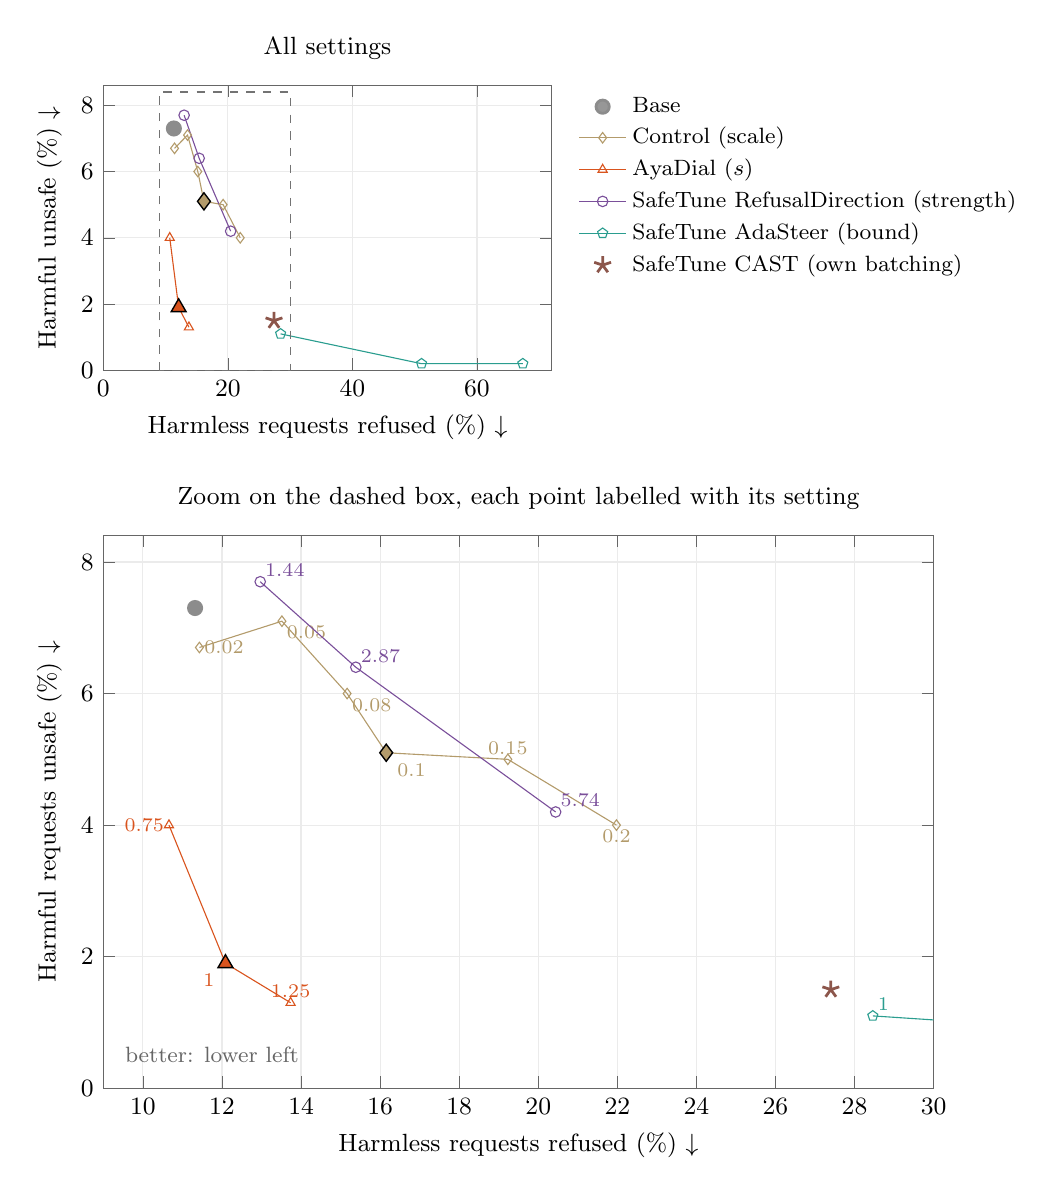
\begin{tikzpicture}
\begin{axis}[name=top, width=0.6\linewidth, height=5.2cm, xmin=0, xmax=72, ymin=0, ymax=8.6,
  xlabel={Harmless requests refused (\%) $\downarrow$}, ylabel={Harmful unsafe (\%) $\downarrow$}, grid=major, grid style={black!8},
  legend style={at={(1.04,1)}, anchor=north west, font=\footnotesize}, legend cell align=left, title={All settings}, title style={font=\small}]
\addplot[only marks, mark=*, mark size=2.4pt, color=cBase] coordinates {(11.319,7.300)};\addlegendentry{Base}
\addplot[color=cCtrl, mark=diamond, mark size=1.9pt, thin, mark options={solid, fill=white}] coordinates {(11.429,6.700) (13.516,7.100) (15.165,6.000) (16.154,5.100) (19.231,5.000) (21.978,4.000)};\addlegendentry{Control (scale)}
\addplot[only marks, color=cCtrl, mark=diamond*, mark size=3.1pt, mark options={draw=black, line width=0.5pt}, forget plot] coordinates {(16.154,5.100)};
\addplot[color=cDial, mark=triangle, mark size=1.9pt, thin, mark options={solid, fill=white}] coordinates {(10.659,4.000) (12.088,1.900) (13.736,1.300)};\addlegendentry{AyaDial ($s$)}
\addplot[only marks, color=cDial, mark=triangle*, mark size=3.1pt, mark options={draw=black, line width=0.5pt}, forget plot] coordinates {(12.088,1.900)};
\addplot[color=cRD, mark=o, mark size=1.9pt, thin, mark options={solid, fill=white}] coordinates {(12.967,7.700) (15.385,6.400) (20.440,4.200)};\addlegendentry{SafeTune RefusalDirection (strength)}
\addplot[color=cAda, mark=pentagon, mark size=1.9pt, thin, mark options={solid, fill=white}] coordinates {(28.462,1.100) (51.099,0.200) (67.363,0.200)};\addlegendentry{SafeTune AdaSteer (bound)}
\addplot[only marks, mark=star, mark size=3.2pt, color=cCast] coordinates {(27.400,1.500)};\addlegendentry{SafeTune CAST (own batching)}
\draw[black!55, dashed] (axis cs:9,0) rectangle (axis cs:30,8.4);
\end{axis}
\begin{axis}[at={(top.south west)}, anchor=north west, yshift=-2.1cm, width=\linewidth, height=8.6cm, xmin=9, xmax=30, ymin=0, ymax=8.4,
  xlabel={Harmless requests refused (\%) $\downarrow$}, ylabel={Harmful requests unsafe (\%) $\downarrow$}, grid=major, grid style={black!8},
  title={Zoom on the dashed box, each point labelled with its setting}, title style={font=\small}, clip=true]
\addplot[only marks, mark=*, mark size=2.4pt, color=cBase] coordinates {(11.319,7.300)};
\addplot[color=cCtrl, mark=diamond, mark size=1.9pt, thin, mark options={solid, fill=white}] coordinates {(11.429,6.700) (13.516,7.100) (15.165,6.000) (16.154,5.100) (19.231,5.000) (21.978,4.000)};
\addplot[only marks, color=cCtrl, mark=diamond*, mark size=3.1pt, mark options={draw=black, line width=0.5pt}, forget plot] coordinates {(16.154,5.100)};
\node[font=\scriptsize, text=cCtrl, anchor=west, inner sep=1.6pt] at (axis cs:11.429,6.700) {0.02};
\node[font=\scriptsize, text=cCtrl, anchor=north west, inner sep=1.6pt] at (axis cs:13.516,7.100) {0.05};
\node[font=\scriptsize, text=cCtrl, anchor=north west, inner sep=1.6pt] at (axis cs:15.165,6.000) {0.08};
\node[font=\scriptsize, text=cCtrl, anchor=north west, inner sep=3.8pt] at (axis cs:16.154,5.100) {0.1};
\node[font=\scriptsize, text=cCtrl, anchor=south, inner sep=1.6pt] at (axis cs:19.231,5.000) {0.15};
\node[font=\scriptsize, text=cCtrl, anchor=north, inner sep=1.6pt] at (axis cs:21.978,4.000) {0.2};
\addplot[color=cDial, mark=triangle, mark size=1.9pt, thin, mark options={solid, fill=white}] coordinates {(10.659,4.000) (12.088,1.900) (13.736,1.300)};
\addplot[only marks, color=cDial, mark=triangle*, mark size=3.1pt, mark options={draw=black, line width=0.5pt}, forget plot] coordinates {(12.088,1.900)};
\node[font=\scriptsize, text=cDial, anchor=east, inner sep=1.6pt] at (axis cs:10.659,4.000) {0.75};
\node[font=\scriptsize, text=cDial, anchor=north east, inner sep=3.8pt] at (axis cs:12.088,1.900) {1};
\node[font=\scriptsize, text=cDial, anchor=south, inner sep=1.6pt] at (axis cs:13.736,1.300) {1.25};
\addplot[color=cRD, mark=o, mark size=1.9pt, thin, mark options={solid, fill=white}] coordinates {(12.967,7.700) (15.385,6.400) (20.440,4.200)};
\node[font=\scriptsize, text=cRD, anchor=south west, inner sep=1.6pt] at (axis cs:12.967,7.700) {1.44};
\node[font=\scriptsize, text=cRD, anchor=south west, inner sep=1.6pt] at (axis cs:15.385,6.400) {2.87};
\node[font=\scriptsize, text=cRD, anchor=south west, inner sep=1.6pt] at (axis cs:20.440,4.200) {5.74};
\addplot[color=cAda, mark=pentagon, mark size=1.9pt, thin, mark options={solid, fill=white}] coordinates {(28.462,1.100) (51.099,0.200) (67.363,0.200)};
\node[font=\scriptsize, text=cAda, anchor=south west, inner sep=1.6pt] at (axis cs:28.462,1.100) {1};
\addplot[only marks, mark=star, mark size=3.2pt, color=cCast] coordinates {(27.400,1.500)};
\node[anchor=south west, font=\footnotesize, text=black!60] at (axis cs:9.3,0.25) {better: lower left};
\end{axis}\end{tikzpicture}
\caption{Unsafe on harmful against refused on harmless, on the WildJailbreak requests of Tables~\ref{tab:mainh} and~\ref{tab:mainb}: each line joins the settings of one method on the same 1910 requests, $s$ is the adapter scale, and filled points with a black outline are the settings in those tables ($s = 1$; Control at 0.1).
SafeTune CAST ran with other batching and its own Base, so it is one point; SafeTune AdaSteer's bounds 2 and 4 lie right of the zoom.}\label{fig:scatter}
\end{figure}
\subsection{The scale $s$}
AyaDial was measured at $s$ = 0.75, 1, 1.25 on the same 1910 WildJailbreak requests. The full sweep from $s = 0$ to 3 was measured on the earlier version of the adapter and is in Appendix~\ref{app:earlier}.
\begin{figure}[H]\centering
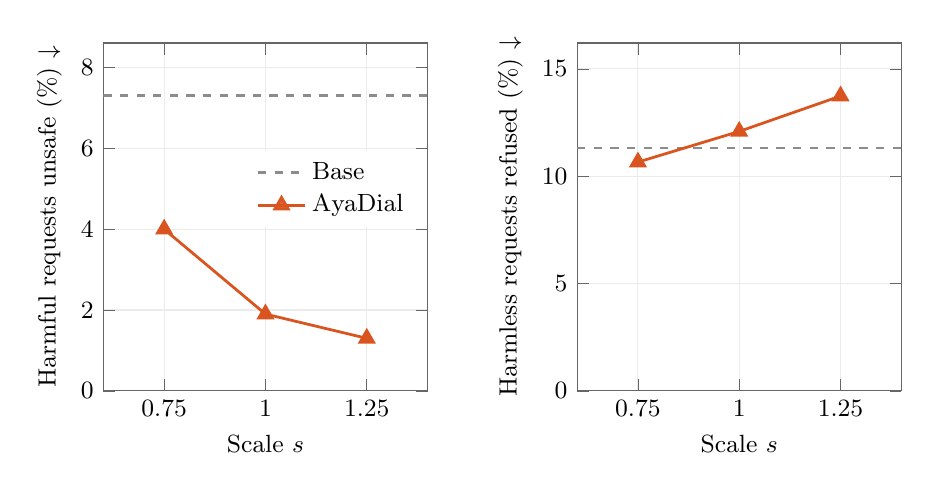
\begin{tikzpicture}
\begin{groupplot}[group style={group size=2 by 1, horizontal sep=1.9cm}, width=0.47\linewidth, height=6cm,
  xmin=0.6, xmax=1.4, xtick={0.75,1,1.25}, xlabel={Scale $s$}, ymin=0, grid=major, grid style={black!8}]
\nextgroupplot[ymax=8.61, ylabel={Harmful requests unsafe (\%) $\downarrow$}, legend style={at={(0.97,0.58)}, anchor=east}, legend cell align=left]
\addplot[color=cBase, dashed, no marks, domain=0.6:1.4] {7.300};\addlegendentry{Base}
\addplot[color=cDial, mark=triangle*, mark size=2.8pt] coordinates {(0.75,4.000) (1,1.900) (1.25,1.300)};\addlegendentry{AyaDial}
\nextgroupplot[ymax=16.21, ylabel={Harmless requests refused (\%) $\downarrow$}]
\addplot[color=cBase, dashed, no marks, domain=0.6:1.4] {11.319};
\addplot[color=cDial, mark=triangle*, mark size=2.8pt] coordinates {(0.75,10.659) (1,12.088) (1.25,13.736)};
\end{groupplot}\end{tikzpicture}
\caption{AyaDial at three settings of $s$, with Base as the dashed line. Unsafe goes from $4.0$\% at $s = 0.75$ to $1.3$\% at $s = 1.25$ while harmless refusal goes from $10.7$\% to $13.7$\%.}\label{fig:dial}
\end{figure}
\section{New requests from known sources}\label{sec:t1}
These are sources that contributed samples to AyaDial's direction, tested on requests and templates it has not seen. They show protection against requests in the style of sources the adapter has samples of.

The requests in this section and in Sections~\ref{sec:t2}, \ref{sec:loosen} and~\ref{sec:open} were set aside before the adapters were computed and were never used to build or tune them; the list of requests and the settings were fixed in advance, and each of the two tests (the first and the second) was run once. They are called unseen requests below. AyaDial's harm direction was computed from WildJailbreak training requests (2500 harmful, 2500 harmless), 620 requests from HarmBench and JailbreakBench plain behaviours, XSTest, Alpaca and OR-Bench-hard, 174 JailbreakBench GCG and PAIR artifacts, 1200 GCG suffix transplants, and half of a separate pool of in-the-wild templates (135) and of MultiJail and Aya requests in 10 languages (426); every request tested here is a different one. Every benchmark that was run, including those where AyaDial is not shown to differ from Control, is in Appendix~\ref{app:all}.

Labels: Qwen3Guard-Gen-0.6B (model judge), for both the refusal and the unsafe label. $\downarrow$ lower is better, $\uparrow$ higher is better. Each benchmark below has its own table. SafeTune RefusalDirection, AdaSteer and CAST were calibrated on the same 7555 requests AyaDial's direction was computed from, and their setting was chosen on development data with the same rule as AyaDial's (RefusalDirection: strength 0.1 added at every layer, SafeTune's default placement; AdaSteer: bound 0.2; CAST: alpha 0.03). AyaDial-WSP is the weight edit of Section~\ref{sec:wsp}, written into the same two units at $s = 1$; it was made after these tests had been opened, on other requests, so its rows are a later run and not a setting fixed in advance.

\begin{figure}[H]\centering
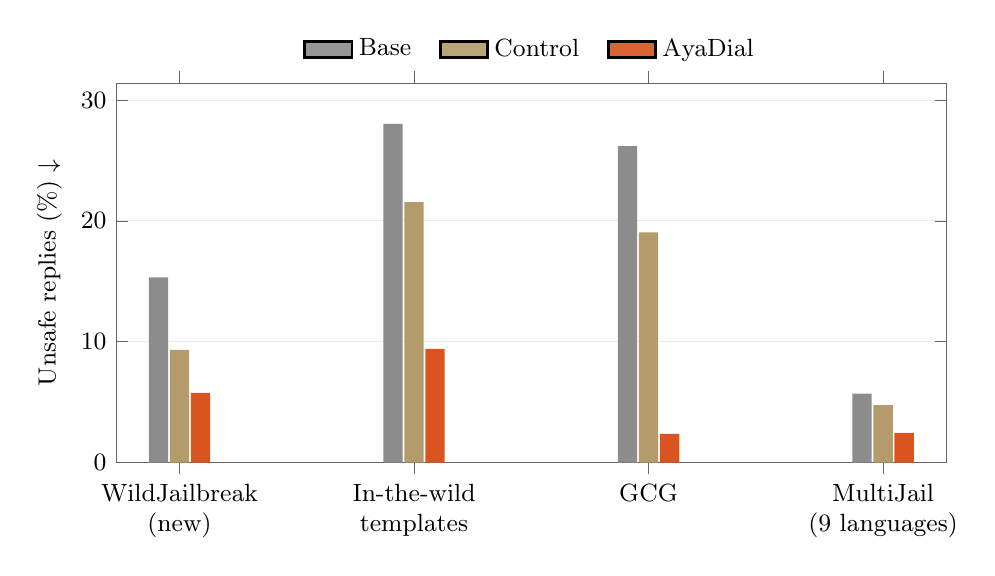
\begin{tikzpicture}
\begin{axis}[ybar=0.6pt, bar width=7pt, width=\linewidth, height=6.4cm, ymin=0, ymax=31.4, enlarge x limits=0.09,
  symbolic x coords={g0,g1,g2,g3}, xtick=data, xticklabels={{WildJailbreak\\(new)},{In-the-wild\\templates},{GCG},{MultiJail\\(9 languages)}},
  xticklabel style={align=center}, ylabel={Unsafe replies (\%) $\downarrow$}, ymajorgrids, grid style={black!8},
  legend style={at={(0.5,1.03)}, anchor=south, legend columns=3, /tikz/every even column/.append style={column sep=8pt}}, legend cell align=left]
\addplot[fill=cBase, draw=none, area legend] coordinates {(g0,15.333) (g1,28.033) (g2,26.190) (g3,5.714)};\addlegendentry{Base}
\addplot[fill=cCtrl, draw=none, area legend] coordinates {(g0,9.333) (g1,21.548) (g2,19.048) (g3,4.762)};\addlegendentry{Control}
\addplot[fill=cDial, draw=none, area legend] coordinates {(g0,5.778) (g1,9.414) (g2,2.381) (g3,2.460)};\addlegendentry{AyaDial}
\end{axis}\end{tikzpicture}
\caption{The four harmful benchmarks of this section at a glance. Compare the last bar of each group (AyaDial) with the second (Control).}\label{fig:t1}
\end{figure}
\needspace{18\baselineskip}\medskip{\raggedright\noindent\large\bfseries Benchmark: WildJailbreak (new requests)\par}\vspace{-3pt}\noindent 450 harmful, 350 harmless requests: jailbreak-wrapped requests from the WildJailbreak benchmark, first test.

\begin{table}[H]\centering\small\renewcommand{\arraystretch}{1.25}\begin{tabular}{|l|r|r|r|l|}\hline
\multicolumn{5}{|l|}{\textbf{Harmful requests ($n = 450$)}}\\\hline
Method & Refused (\%) $\uparrow$ & \makecell[r]{Answered without\\harm (\%)} & Unsafe (\%) $\downarrow$ & \makecell[l]{Unsafe, difference from\\Control (95\% interval)}\\\hline
Base & $72.4$ & $12.2$ & $15.3$ & \\\hline
Control & $78.4$ & $12.2$ & $9.3$ & \\\hline
AyaDial & $86.0$ & $8.2$ & $5.8$ & $-3.6$\,[$-6.2$, $-0.9$]\\\hline
AyaDial-WSP & \cellcolor{win}$\mathbf{89.1}$ & $6.9$ & \cellcolor{win}$\mathbf{4.0}$ & \\\hline
SafeTune RefusalDirection & $75.8$ & $12.4$ & $11.8$ & \\\hline
SafeTune AdaSteer & $77.8$ & $12.7$ & $9.6$ & \\\hline
SafeTune CAST & $77.8$ & $11.3$ & $10.9$ & \\\hline
\end{tabular}\end{table}
\begin{table}[H]\centering\small\renewcommand{\arraystretch}{1.25}\begin{tabular}{|l|r|r|l|}\hline
\multicolumn{4}{|l|}{\textbf{Harmless requests ($n = 350$)}}\\\hline
Method & Refused (\%) $\downarrow$ & Answered (\%) $\uparrow$ & \makecell[l]{Refused, difference from\\Control (95\% interval)}\\\hline
Base & $8.6$ & $91.4$ & \\\hline
Control & $12.0$ & $88.0$ & \\\hline
AyaDial & $9.7$ & $90.3$ & $-2.3$\,[$-5.1$, $0.6$]\\\hline
AyaDial-WSP & $11.7$ & $88.3$ & \\\hline
SafeTune RefusalDirection & $10.3$ & $89.7$ & \\\hline
SafeTune AdaSteer & $9.7$ & $90.3$ & \\\hline
SafeTune CAST & $9.1$ & $90.9$ & \\\hline
\end{tabular}\end{table}
Unsafe, AyaDial against Control: $-3.6$\,[$-6.2$, $-0.9$], established against Control (the interval excludes 0).

\needspace{18\baselineskip}\medskip{\raggedright\noindent\large\bfseries Benchmark: in-the-wild jailbreak templates\par}\vspace{-3pt}\noindent 478 harmful, 239 harmless requests: jailbreak prompts collected from online communities, with a harmful question or a harmless instruction, first test.

\begin{table}[H]\centering\small\renewcommand{\arraystretch}{1.25}\begin{tabular}{|l|r|r|r|l|}\hline
\multicolumn{5}{|l|}{\textbf{Harmful requests ($n = 478$)}}\\\hline
Method & Refused (\%) $\uparrow$ & \makecell[r]{Answered without\\harm (\%)} & Unsafe (\%) $\downarrow$ & \makecell[l]{Unsafe, difference from\\Control (95\% interval)}\\\hline
Base & $67.6$ & $4.4$ & $28.0$ & \\\hline
Control & $75.9$ & $2.5$ & $21.5$ & \\\hline
AyaDial & $87.7$ & $2.9$ & \cellcolor{win}$\mathbf{9.4}$ & $-12.1$\,[$-15.9$, $-8.2$]\\\hline
AyaDial-WSP & \cellcolor{win}$\mathbf{88.1}$ & $2.5$ & \cellcolor{win}$\mathbf{9.4}$ & \\\hline
SafeTune RefusalDirection & $70.5$ & $4.0$ & $25.5$ & \\\hline
SafeTune AdaSteer & $76.2$ & $2.9$ & $20.9$ & \\\hline
SafeTune CAST & $74.5$ & $3.6$ & $22.0$ & \\\hline
\end{tabular}\end{table}
\begin{table}[H]\centering\small\renewcommand{\arraystretch}{1.25}\begin{tabular}{|l|r|r|l|}\hline
\multicolumn{4}{|l|}{\textbf{Harmless requests ($n = 239$)}}\\\hline
Method & Refused (\%) $\downarrow$ & Answered (\%) $\uparrow$ & \makecell[l]{Refused, difference from\\Control (95\% interval)}\\\hline
Base & $15.5$ & $84.5$ & \\\hline
Control & $20.1$ & $79.9$ & \\\hline
AyaDial & $20.5$ & $79.5$ & $+0.4$\,[$-4.2$, $5.0$]\\\hline
AyaDial-WSP & \cellcolor{win}$\mathbf{17.6}$ & \cellcolor{win}$\mathbf{82.4}$ & \\\hline
SafeTune RefusalDirection & $19.7$ & $80.3$ & \\\hline
SafeTune AdaSteer & $20.5$ & $79.5$ & \\\hline
SafeTune CAST & $18.8$ & $81.2$ & \\\hline
\end{tabular}\end{table}
Unsafe, AyaDial against Control: $-12.1$\,[$-15.9$, $-8.2$], established against Control (the interval excludes 0).

\needspace{18\baselineskip}\medskip{\raggedright\noindent\large\bfseries Benchmark: JailbreakBench GCG\par}\vspace{-3pt}\noindent 42 harmful, 100 harmless requests: an optimised attack suffix on behaviours AyaDial never saw; the harmless set carries a transplanted suffix, first test.

\begin{table}[H]\centering\small\renewcommand{\arraystretch}{1.25}\begin{tabular}{|l|r|r|r|l|}\hline
\multicolumn{5}{|l|}{\textbf{Harmful requests ($n = 42$)}}\\\hline
Method & Refused (\%) $\uparrow$ & \makecell[r]{Answered without\\harm (\%)} & Unsafe (\%) $\downarrow$ & \makecell[l]{Unsafe, difference from\\Control (95\% interval)}\\\hline
Base & $69.0$ & $4.8$ & $26.2$ & \\\hline
Control & $73.8$ & $7.1$ & $19.0$ & \\\hline
AyaDial & \cellcolor{win}$\mathbf{92.9}$ & $4.8$ & \cellcolor{win}$\mathbf{2.4}$ & $-16.7$\,[$-28.6$, $-7.1$]\\\hline
AyaDial-WSP & $88.1$ & $7.1$ & $4.8$ & \\\hline
SafeTune RefusalDirection & $71.4$ & $11.9$ & $16.7$ & \\\hline
SafeTune AdaSteer & $73.8$ & $7.1$ & $19.0$ & \\\hline
SafeTune CAST & $73.8$ & $9.5$ & $16.7$ & \\\hline
\end{tabular}\end{table}
\begin{table}[H]\centering\small\renewcommand{\arraystretch}{1.25}\begin{tabular}{|l|r|r|l|}\hline
\multicolumn{4}{|l|}{\textbf{Harmless requests ($n = 100$)}}\\\hline
Method & Refused (\%) $\downarrow$ & Answered (\%) $\uparrow$ & \makecell[l]{Refused, difference from\\Control (95\% interval)}\\\hline
Base & $1.0$ & $99.0$ & \\\hline
Control & $1.0$ & $99.0$ & \\\hline
AyaDial & $2.0$ & $98.0$ & $+1.0$\,[$0.0$, $3.0$]\\\hline
AyaDial-WSP & $1.0$ & $99.0$ & \\\hline
SafeTune RefusalDirection & $2.0$ & $98.0$ & \\\hline
SafeTune AdaSteer & $1.0$ & $99.0$ & \\\hline
SafeTune CAST & $1.0$ & $99.0$ & \\\hline
\end{tabular}\end{table}
Unsafe, AyaDial against Control: $-16.7$\,[$-28.6$, $-7.1$], established against Control (the interval excludes 0).

\needspace{18\baselineskip}\medskip{\raggedright\noindent\large\bfseries Benchmark: MultiJail, 9 languages\par}\vspace{-3pt}\noindent 1260 harmful, 625 harmless requests: harmful questions in nine non-English languages, with Aya prompts in the same languages as the harmless set, first test.

\begin{table}[H]\centering\small\renewcommand{\arraystretch}{1.25}\begin{tabular}{|l|r|r|r|l|}\hline
\multicolumn{5}{|l|}{\textbf{Harmful requests ($n = 1260$)}}\\\hline
Method & Refused (\%) $\uparrow$ & \makecell[r]{Answered without\\harm (\%)} & Unsafe (\%) $\downarrow$ & \makecell[l]{Unsafe, difference from\\Control (95\% interval)}\\\hline
Base & $53.1$ & $41.2$ & $5.7$ & \\\hline
Control & $56.7$ & $38.6$ & $4.8$ & \\\hline
AyaDial & $68.7$ & $28.9$ & \cellcolor{win}$\mathbf{2.5}$ & $-2.3$\,[$-3.3$, $-1.4$]\\\hline
AyaDial-WSP & \cellcolor{win}$\mathbf{69.4}$ & $27.9$ & $2.7$ & \\\hline
SafeTune RefusalDirection & $55.2$ & $39.8$ & $4.9$ & \\\hline
SafeTune AdaSteer & $55.6$ & $40.0$ & $4.4$ & \\\hline
SafeTune CAST & $56.3$ & $39.1$ & $4.6$ & \\\hline
\end{tabular}\end{table}
\begin{table}[H]\centering\small\renewcommand{\arraystretch}{1.25}\begin{tabular}{|l|r|r|l|}\hline
\multicolumn{4}{|l|}{\textbf{Harmless requests ($n = 625$)}}\\\hline
Method & Refused (\%) $\downarrow$ & Answered (\%) $\uparrow$ & \makecell[l]{Refused, difference from\\Control (95\% interval)}\\\hline
Base & $1.3$ & $98.7$ & \\\hline
Control & $1.6$ & $98.4$ & \\\hline
AyaDial & $1.9$ & $98.1$ & $+0.3$\,[$-0.3$, $1.1$]\\\hline
AyaDial-WSP & $1.8$ & $98.2$ & \\\hline
SafeTune RefusalDirection & $1.6$ & $98.4$ & \\\hline
SafeTune AdaSteer & $1.3$ & $98.7$ & \\\hline
SafeTune CAST & $1.3$ & $98.7$ & \\\hline
\end{tabular}\end{table}
Unsafe, AyaDial against Control: $-2.3$\,[$-3.3$, $-1.4$], established against Control (the interval excludes 0).

\section{Benchmarks never seen}\label{sec:t2}
No sample of these sources entered any computation of AyaDial. They test whether its harm score carries over to kinds of requests it has never met.

Labels: Qwen3Guard-Gen-0.6B (model judge), for both the refusal and the unsafe label. $\downarrow$ lower is better, $\uparrow$ higher is better. Each benchmark below has its own table. SafeTune RefusalDirection, AdaSteer and CAST were calibrated on the same 7555 requests AyaDial's direction was computed from, and their setting was chosen on development data with the same rule as AyaDial's (RefusalDirection: strength 0.1 added at every layer, SafeTune's default placement; AdaSteer: bound 0.2; CAST: alpha 0.03). AyaDial-WSP is the weight edit of Section~\ref{sec:wsp}, written into the same two units at $s = 1$; it was made after these tests had been opened, on other requests, so its rows are a later run and not a setting fixed in advance.

\needspace{18\baselineskip}\medskip{\raggedright\noindent\large\bfseries Benchmark: Aya red-teaming, six languages\par}\vspace{-3pt}\noindent 900 harmful, 360 harmless requests: harmful requests written by native speakers in Filipino, French, Hindi, Russian, Serbian and Spanish, second test; the harmless set is Aya prompts in the same languages, from a source AyaDial saw in ten other languages.

\begin{table}[H]\centering\small\renewcommand{\arraystretch}{1.25}\begin{tabular}{|l|r|r|r|l|}\hline
\multicolumn{5}{|l|}{\textbf{Harmful requests ($n = 900$)}}\\\hline
Method & Refused (\%) $\uparrow$ & \makecell[r]{Answered without\\harm (\%)} & Unsafe (\%) $\downarrow$ & \makecell[l]{Unsafe, difference from\\Control (95\% interval)}\\\hline
Base & $56.8$ & $31.0$ & $12.2$ & \\\hline
Control & $61.0$ & $28.1$ & $10.9$ & \\\hline
AyaDial & $71.2$ & $21.0$ & $7.8$ & $-3.1$\,[$-4.4$, $-1.7$]\\\hline
AyaDial-WSP & \cellcolor{win}$\mathbf{76.4}$ & $18.7$ & \cellcolor{win}$\mathbf{4.9}$ & \\\hline
SafeTune RefusalDirection & $58.1$ & $30.0$ & $11.9$ & \\\hline
SafeTune AdaSteer & $60.0$ & $29.6$ & $10.4$ & \\\hline
SafeTune CAST & $59.9$ & $28.8$ & $11.3$ & \\\hline
\end{tabular}\end{table}
\begin{table}[H]\centering\small\renewcommand{\arraystretch}{1.25}\begin{tabular}{|l|r|r|l|}\hline
\multicolumn{4}{|l|}{\textbf{Harmless requests ($n = 360$)}}\\\hline
Method & Refused (\%) $\downarrow$ & Answered (\%) $\uparrow$ & \makecell[l]{Refused, difference from\\Control (95\% interval)}\\\hline
Base & $0.8$ & $99.2$ & \\\hline
Control & $1.1$ & $98.9$ & \\\hline
AyaDial & $0.8$ & $99.2$ & $-0.3$\,[$-0.8$, $0.0$]\\\hline
AyaDial-WSP & $0.8$ & $99.2$ & \\\hline
SafeTune RefusalDirection & $1.1$ & $98.9$ & \\\hline
SafeTune AdaSteer & $0.8$ & $99.2$ & \\\hline
SafeTune CAST & $0.8$ & $99.2$ & \\\hline
\end{tabular}\end{table}
Unsafe, AyaDial against Control: $-3.1$\,[$-4.4$, $-1.7$], established against Control (the interval excludes 0). A second judge, Qwen3Guard-Gen-8B, gives $9.2$\% to $5.9$\% unsafe ($-2.6$\,[$-4.0$, $-1.2$] against Control).

\begin{figure}[H]\centering
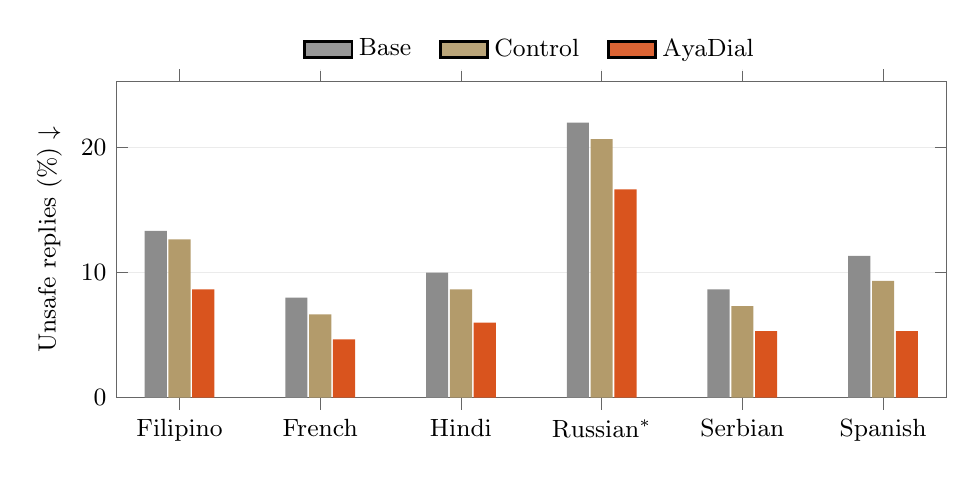
\begin{tikzpicture}
\begin{axis}[ybar=0.6pt, bar width=8pt, width=\linewidth, height=5.6cm, ymin=0, ymax=25.3, enlarge x limits=0.09,
  symbolic x coords={l0,l1,l2,l3,l4,l5}, xtick=data, xticklabels={{Filipino},{French},{Hindi},{Russian$^{*}$},{Serbian},{Spanish}},
  ylabel={Unsafe replies (\%) $\downarrow$}, ymajorgrids, grid style={black!8},
  legend style={at={(0.5,1.03)}, anchor=south, legend columns=3, /tikz/every even column/.append style={column sep=8pt}}, legend cell align=left]
\addplot[fill=cBase, draw=none, area legend] coordinates {(l0,13.333) (l1,8.000) (l2,10.000) (l3,22.000) (l4,8.667) (l5,11.333)};\addlegendentry{Base}
\addplot[fill=cCtrl, draw=none, area legend] coordinates {(l0,12.667) (l1,6.667) (l2,8.667) (l3,20.667) (l4,7.333) (l5,9.333)};\addlegendentry{Control}
\addplot[fill=cDial, draw=none, area legend] coordinates {(l0,8.667) (l1,4.667) (l2,6.000) (l3,16.667) (l4,5.333) (l5,5.333)};\addlegendentry{AyaDial}
\end{axis}\end{tikzpicture}
\caption{Unsafe replies per language, 150 harmful requests each (second test). Only Russian$^{*}$ has an interval against Control that excludes 0 (Russian $-4.0$\,[$-7.3$, $-1.3$]), so the pooled result is the claim.}\label{fig:langs}
\end{figure}
\needspace{18\baselineskip}\medskip{\raggedright\noindent\large\bfseries Benchmark: JailbreakBench random search\par}\vspace{-3pt}\noindent 77 harmful requests: an attack method AyaDial never saw, run on behaviours it never saw, first test.

\begin{table}[H]\centering\small\renewcommand{\arraystretch}{1.25}\begin{tabular}{|l|r|r|r|l|}\hline
\multicolumn{5}{|l|}{\textbf{Harmful requests ($n = 77$)}}\\\hline
Method & Refused (\%) $\uparrow$ & \makecell[r]{Answered without\\harm (\%)} & Unsafe (\%) $\downarrow$ & \makecell[l]{Unsafe, difference from\\Control (95\% interval)}\\\hline
Base & $23.4$ & $5.2$ & $71.4$ & \\\hline
Control & $41.6$ & $5.2$ & $53.2$ & \\\hline
AyaDial & $77.9$ & $5.2$ & $16.9$ & $-36.4$\,[$-53.8$, $-19.7$]\\\hline
AyaDial-WSP & \cellcolor{win}$\mathbf{85.7}$ & $5.2$ & \cellcolor{win}$\mathbf{9.1}$ & \\\hline
SafeTune RefusalDirection & $41.6$ & $5.2$ & $53.2$ & \\\hline
SafeTune AdaSteer & $54.5$ & $6.5$ & $39.0$ & \\\hline
SafeTune CAST & $36.4$ & $5.2$ & $58.4$ & \\\hline
\end{tabular}\end{table}
Unsafe, AyaDial against Control: $-36.4$\,[$-53.8$, $-19.7$], established against Control (the interval excludes 0).

\needspace{18\baselineskip}\medskip{\raggedright\noindent\large\bfseries Benchmark: SORRY-Bench, base questions\par}\vspace{-3pt}\noindent 334 harmful requests: harmful questions asked plainly, first test.

\begin{table}[H]\centering\small\renewcommand{\arraystretch}{1.25}\begin{tabular}{|l|r|r|r|l|}\hline
\multicolumn{5}{|l|}{\textbf{Harmful requests ($n = 334$)}}\\\hline
Method & Refused (\%) $\uparrow$ & \makecell[r]{Answered without\\harm (\%)} & Unsafe (\%) $\downarrow$ & \makecell[l]{Unsafe, difference from\\Control (95\% interval)}\\\hline
Base & $69.5$ & $15.6$ & $15.0$ & \\\hline
Control & $74.0$ & $15.3$ & $10.8$ & \\\hline
AyaDial & \cellcolor{win}$\mathbf{78.1}$ & $13.2$ & \cellcolor{win}$\mathbf{8.7}$ & $-2.1$\,[$-5.1$, $0.9$]\\\hline
AyaDial-WSP & $77.5$ & $12.6$ & $9.9$ & \\\hline
SafeTune RefusalDirection & $71.9$ & $16.2$ & $12.0$ & \\\hline
SafeTune AdaSteer & $71.0$ & $15.6$ & $13.5$ & \\\hline
SafeTune CAST & $71.9$ & $15.0$ & $13.2$ & \\\hline
\end{tabular}\end{table}
Unsafe, AyaDial against Control: $-2.1$\,[$-5.1$, $0.9$], lower than Base, not shown to differ from Control.

\needspace{18\baselineskip}\medskip{\raggedright\noindent\large\bfseries Benchmark: SORRY-Bench, other styles\par}\vspace{-3pt}\noindent 760 harmful requests: the same kind of questions rewritten in 20 styles (persuasion, role play, misspellings, ciphers, translations), first test.

\begin{table}[H]\centering\small\renewcommand{\arraystretch}{1.25}\begin{tabular}{|l|r|r|r|l|}\hline
\multicolumn{5}{|l|}{\textbf{Harmful requests ($n = 760$)}}\\\hline
Method & Refused (\%) $\uparrow$ & \makecell[r]{Answered without\\harm (\%)} & Unsafe (\%) $\downarrow$ & \makecell[l]{Unsafe, difference from\\Control (95\% interval)}\\\hline
Base & $39.1$ & $49.2$ & $11.7$ & \\\hline
Control & $42.8$ & $47.1$ & $10.1$ & \\\hline
AyaDial & $46.4$ & $44.2$ & $9.3$ & $-0.8$\,[$-2.4$, $0.9$]\\\hline
AyaDial-WSP & \cellcolor{win}$\mathbf{52.0}$ & $39.9$ & \cellcolor{win}$\mathbf{8.2}$ & \\\hline
SafeTune RefusalDirection & $40.8$ & $47.4$ & $11.8$ & \\\hline
SafeTune AdaSteer & $41.3$ & $47.1$ & $11.6$ & \\\hline
SafeTune CAST & $41.8$ & $47.1$ & $11.1$ & \\\hline
\end{tabular}\end{table}
Unsafe, AyaDial against Control: $-0.8$\,[$-2.4$, $0.9$], lower than Base, not shown to differ from Control.

\needspace{18\baselineskip}\medskip{\raggedright\noindent\large\bfseries Benchmark: PHTest\par}\vspace{-3pt}\noindent 449 harmless requests: harmless requests that look harmful, first test.

\begin{table}[H]\centering\small\renewcommand{\arraystretch}{1.25}\begin{tabular}{|l|r|r|l|}\hline
\multicolumn{4}{|l|}{\textbf{Harmless requests ($n = 449$)}}\\\hline
Method & Refused (\%) $\downarrow$ & Answered (\%) $\uparrow$ & \makecell[l]{Refused, difference from\\Control (95\% interval)}\\\hline
Base & $6.0$ & $94.0$ & \\\hline
Control & $8.2$ & $91.8$ & \\\hline
AyaDial & $7.6$ & $92.4$ & $-0.7$\,[$-2.7$, $1.6$]\\\hline
AyaDial-WSP & $7.1$ & $92.9$ & \\\hline
SafeTune RefusalDirection & $7.6$ & $92.4$ & \\\hline
SafeTune AdaSteer & $6.5$ & $93.5$ & \\\hline
SafeTune CAST & $7.8$ & $92.2$ & \\\hline
\end{tabular}\end{table}
Refused, AyaDial against Control: $-0.7$\,[$-2.7$, $1.6$], not shown to differ from Control; against Base: $+1.6$\,[$0.2$, $3.1$], higher than Base.

\section{Open problem: system prompts and multi-turn chats}\label{sec:open}
In real use a model sits behind a developer's system prompt or inside a longer conversation. In those formats AyaDial lowers unsafe replies against Base ($-5.3$\,[$-8.3$, $-2.5$] points) but is not shown to differ from Control ($+0.2$\,[$-3.0$, $3.3$]), while it avoids Control's extra refusals of harmless requests ($-2.9$\,[$-5.0$, $-1.0$] against Control, $-0.1$\,[$-1.0$, $0.8$] against Base). The measured reason: on a separate set of requests, AyaDial's harm score passes its threshold on $92.5$\% of harmful requests in the default format and on $57.5$\% behind a long system prompt. Section~\ref{sec:wsp} shows what a weight edit written by a frontier LLM did on this problem.

Harmful requests come from WildJailbreak and MultiJail English, harmless requests from OR-Bench-hard, Alpaca and WildJailbreak; they are unseen requests from the second test.

Labels: Qwen3Guard-Gen-0.6B (model judge), for both the refusal and the unsafe label. $\downarrow$ lower is better, $\uparrow$ higher is better. Each benchmark below has its own table. SafeTune RefusalDirection, AdaSteer and CAST were calibrated on the same 7555 requests AyaDial's direction was computed from, and their setting was chosen on development data with the same rule as AyaDial's (RefusalDirection: strength 0.1 added at every layer, SafeTune's default placement; AdaSteer: bound 0.2; CAST: alpha 0.03). AyaDial-WSP is the weight edit of Section~\ref{sec:wsp}, written into the same two units at $s = 1$; it was made after these tests had been opened, on other requests, so its rows are a later run and not a setting fixed in advance.

\begin{figure}[H]\centering
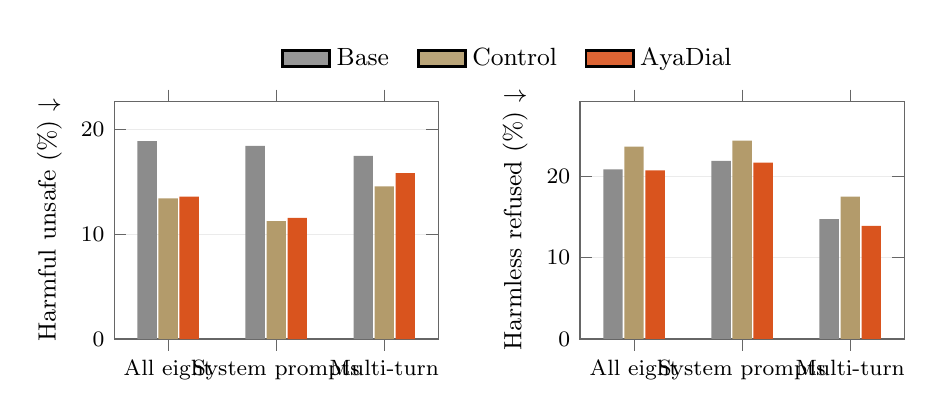
\begin{tikzpicture}
\begin{groupplot}[group style={group size=2 by 1, horizontal sep=1.8cm}, width=0.47\linewidth, height=4.6cm,
  enlarge x limits=0.25, ymajorgrids, grid style={black!8}, tick label style={font=\footnotesize}]
\nextgroupplot[ybar=0.6pt, bar width=7pt, symbolic x coords={f0,f1,f2}, xtick=data, xticklabels={{All eight},{System prompts},{Multi-turn}}, ymin=0, ymax=22.7, ylabel={Harmful unsafe (\%) $\downarrow$}, legend to name=fmtleg, legend columns=3, legend style={/tikz/every even column/.append style={column sep=8pt}}]
\addplot[fill=cBase, draw=none, area legend] coordinates {(f0,18.906) (f1,18.438) (f2,17.500)};\addlegendentry{Base}
\addplot[fill=cCtrl, draw=none, area legend] coordinates {(f0,13.438) (f1,11.250) (f2,14.583)};\addlegendentry{Control}
\addplot[fill=cDial, draw=none, area legend] coordinates {(f0,13.594) (f1,11.562) (f2,15.833)};\addlegendentry{AyaDial}
\nextgroupplot[ybar=0.6pt, bar width=7pt, symbolic x coords={f0,f1,f2}, xtick=data, xticklabels={{All eight},{System prompts},{Multi-turn}}, ymin=0, ymax=29.2, ylabel={Harmless refused (\%) $\downarrow$}]
\addplot[fill=cBase, draw=none, area legend] coordinates {(f0,20.833) (f1,21.875) (f2,14.722)};
\addplot[fill=cCtrl, draw=none, area legend] coordinates {(f0,23.646) (f1,24.375) (f2,17.500)};
\addplot[fill=cDial, draw=none, area legend] coordinates {(f0,20.729) (f1,21.667) (f2,13.889)};
\end{groupplot}
\node[anchor=south] at ($(group c1r1.north)!0.5!(group c2r1.north)+(0,4pt)$) {\pgfplotslegendfromname{fmtleg}};
\end{tikzpicture}
\caption{The three format blocks below at a glance: harmful requests on the left, harmless on the right.}\label{fig:fmt}
\end{figure}
\needspace{18\baselineskip}\medskip{\raggedright\noindent\large\bfseries Benchmark: all eight formats\par}\vspace{-3pt}\noindent 640 harmful, 960 harmless requests: four system prompts, three multi-turn chats and one in-the-wild template as the system prompt.

\begin{table}[H]\centering\small\renewcommand{\arraystretch}{1.25}\begin{tabular}{|l|r|r|r|l|}\hline
\multicolumn{5}{|l|}{\textbf{Harmful requests ($n = 640$)}}\\\hline
Method & Refused (\%) $\uparrow$ & \makecell[r]{Answered without\\harm (\%)} & Unsafe (\%) $\downarrow$ & \makecell[l]{Unsafe, difference from\\Control (95\% interval)}\\\hline
Base & $61.4$ & $19.7$ & $18.9$ & \\\hline
Control & $69.5$ & $17.0$ & $13.4$ & \\\hline
AyaDial & $68.8$ & $17.7$ & $13.6$ & $+0.2$\,[$-3.0$, $3.3$]\\\hline
AyaDial-WSP & \cellcolor{win}$\mathbf{72.2}$ & $16.7$ & \cellcolor{win}$\mathbf{11.1}$ & \\\hline
SafeTune RefusalDirection & $63.9$ & $17.8$ & $18.3$ & \\\hline
SafeTune AdaSteer & $65.6$ & $18.4$ & $15.9$ & \\\hline
SafeTune CAST & $63.4$ & $19.2$ & $17.3$ & \\\hline
\end{tabular}\end{table}
\begin{table}[H]\centering\small\renewcommand{\arraystretch}{1.25}\begin{tabular}{|l|r|r|l|}\hline
\multicolumn{4}{|l|}{\textbf{Harmless requests ($n = 960$)}}\\\hline
Method & Refused (\%) $\downarrow$ & Answered (\%) $\uparrow$ & \makecell[l]{Refused, difference from\\Control (95\% interval)}\\\hline
Base & $20.8$ & $79.2$ & \\\hline
Control & $23.6$ & $76.4$ & \\\hline
AyaDial & $20.7$ & $79.3$ & $-2.9$\,[$-5.0$, $-1.0$]\\\hline
AyaDial-WSP & $22.0$ & $78.0$ & \\\hline
SafeTune RefusalDirection & $23.0$ & $77.0$ & \\\hline
SafeTune AdaSteer & $21.9$ & $78.1$ & \\\hline
SafeTune CAST & $21.6$ & $78.4$ & \\\hline
\end{tabular}\end{table}
Unsafe, AyaDial against Control: $+0.2$\,[$-3.0$, $3.3$], lower than Base, not shown to differ from Control.

\needspace{18\baselineskip}\medskip{\raggedright\noindent\large\bfseries Benchmark: four system prompts\par}\vspace{-3pt}\noindent 320 harmful, 480 harmless requests: the request placed behind one of four system prompts.

\begin{table}[H]\centering\small\renewcommand{\arraystretch}{1.25}\begin{tabular}{|l|r|r|r|l|}\hline
\multicolumn{5}{|l|}{\textbf{Harmful requests ($n = 320$)}}\\\hline
Method & Refused (\%) $\uparrow$ & \makecell[r]{Answered without\\harm (\%)} & Unsafe (\%) $\downarrow$ & \makecell[l]{Unsafe, difference from\\Control (95\% interval)}\\\hline
Base & $63.1$ & $18.4$ & $18.4$ & \\\hline
Control & $73.4$ & $15.3$ & $11.2$ & \\\hline
AyaDial & $70.6$ & $17.8$ & $11.6$ & $+0.3$\,[$-3.8$, $4.1$]\\\hline
AyaDial-WSP & \cellcolor{win}$\mathbf{75.3}$ & $14.7$ & \cellcolor{win}$\mathbf{10.0}$ & \\\hline
SafeTune RefusalDirection & $63.8$ & $18.1$ & $18.1$ & \\\hline
SafeTune AdaSteer & $68.4$ & $16.9$ & $14.7$ & \\\hline
SafeTune CAST & $65.0$ & $18.8$ & $16.2$ & \\\hline
\end{tabular}\end{table}
\begin{table}[H]\centering\small\renewcommand{\arraystretch}{1.25}\begin{tabular}{|l|r|r|l|}\hline
\multicolumn{4}{|l|}{\textbf{Harmless requests ($n = 480$)}}\\\hline
Method & Refused (\%) $\downarrow$ & Answered (\%) $\uparrow$ & \makecell[l]{Refused, difference from\\Control (95\% interval)}\\\hline
Base & $21.9$ & $78.1$ & \\\hline
Control & $24.4$ & $75.6$ & \\\hline
AyaDial & \cellcolor{win}$\mathbf{21.7}$ & \cellcolor{win}$\mathbf{78.3}$ & $-2.7$\,[$-5.4$, $-0.2$]\\\hline
AyaDial-WSP & $23.3$ & $76.7$ & \\\hline
SafeTune RefusalDirection & $22.9$ & $77.1$ & \\\hline
SafeTune AdaSteer & $22.7$ & $77.3$ & \\\hline
SafeTune CAST & $22.7$ & $77.3$ & \\\hline
\end{tabular}\end{table}
Unsafe, AyaDial against Control: $+0.3$\,[$-3.8$, $4.1$], lower than Base, not shown to differ from Control.

\needspace{18\baselineskip}\medskip{\raggedright\noindent\large\bfseries Benchmark: three multi-turn chats\par}\vspace{-3pt}\noindent 240 harmful, 360 harmless requests: the request placed after earlier turns of a conversation.

\begin{table}[H]\centering\small\renewcommand{\arraystretch}{1.25}\begin{tabular}{|l|r|r|r|l|}\hline
\multicolumn{5}{|l|}{\textbf{Harmful requests ($n = 240$)}}\\\hline
Method & Refused (\%) $\uparrow$ & \makecell[r]{Answered without\\harm (\%)} & Unsafe (\%) $\downarrow$ & \makecell[l]{Unsafe, difference from\\Control (95\% interval)}\\\hline
Base & $56.7$ & $25.8$ & $17.5$ & \\\hline
Control & $62.5$ & $22.9$ & $14.6$ & \\\hline
AyaDial & $62.1$ & $22.1$ & $15.8$ & $+1.2$\,[$-2.9$, $5.4$]\\\hline
AyaDial-WSP & \cellcolor{win}$\mathbf{63.8}$ & $23.8$ & \cellcolor{win}$\mathbf{12.5}$ & \\\hline
SafeTune RefusalDirection & $60.4$ & $22.1$ & $17.5$ & \\\hline
SafeTune AdaSteer & $58.3$ & $25.0$ & $16.7$ & \\\hline
SafeTune CAST & $57.9$ & $24.6$ & $17.5$ & \\\hline
\end{tabular}\end{table}
\begin{table}[H]\centering\small\renewcommand{\arraystretch}{1.25}\begin{tabular}{|l|r|r|l|}\hline
\multicolumn{4}{|l|}{\textbf{Harmless requests ($n = 360$)}}\\\hline
Method & Refused (\%) $\downarrow$ & Answered (\%) $\uparrow$ & \makecell[l]{Refused, difference from\\Control (95\% interval)}\\\hline
Base & $14.7$ & $85.3$ & \\\hline
Control & $17.5$ & $82.5$ & \\\hline
AyaDial & \cellcolor{win}$\mathbf{13.9}$ & \cellcolor{win}$\mathbf{86.1}$ & $-3.6$\,[$-6.4$, $-1.1$]\\\hline
AyaDial-WSP & $15.3$ & $84.7$ & \\\hline
SafeTune RefusalDirection & $17.8$ & $82.2$ & \\\hline
SafeTune AdaSteer & $15.6$ & $84.4$ & \\\hline
SafeTune CAST & $15.0$ & $85.0$ & \\\hline
\end{tabular}\end{table}
Unsafe, AyaDial against Control: $+1.2$\,[$-2.9$, $5.4$], not shown to differ from Base or Control.

\section{Weight-space programming}\label{sec:wsp}
Weight-space programming (WSP) means letting a language model read and write another network's weights directly. A frontier LLM, Claude Fable 5.2 at maximum reasoning effort, was given AyaDial's construction and scores as facts and asked to improve it, with no instruction on what to fix. It worked blind: it saw only the harness's messages, numbers and request ids, never the text of a request or a reply; it ran its own Python code on the weights of layers 18 to 22 in a sandbox with no network, and could ask for forward passes on a GPU (35 of 40 read passes and 7 of 12 generate-and-judge passes used). There was no gradient training, only closed-form linear algebra; the run took 155 turns, 104 Python runs and \$39.05, and ended at the \$50 cap. The setup follows \emph{Sparks of Weight-Space Programming} (Takehi, Teoh, Zhang and Khattab, 2026, a blog post, \url{https://rikiyat.github.io/blog/weight-space-programming/}).

What it found: under a long system prompt the harm score of harmful requests drops (by 0.28 on average, against 0.08 for harmless ones) and its direction rotates (cosine 0.85 with the default one), and the position guard leaks at the reply-start token, so a threshold change is not enough.

Two edits are compared with AyaDial on the same requests in the same batch, all at $s = 1$. \textbf{AyaDial-WSP} keeps AyaDial's two units and replaces their harm direction with one the editor recomputed from activations in 14 prompt formats (threshold 0.60). \textbf{AyaDial-WSP (add-on)}, the editor's final edit, leaves AyaDial's two units untouched and adds a second pair of units that opens only under system prompts and in multi-turn chats. The editor moved from the first design to the second because of our rule that no harmless group may be refused more than 2 points above the starting adapter (an intermediate candidate fired on 10 of 284 unread multilingual harmless prompts against 4 for AyaDial); our own comparison afterwards favours the first on unsafe replies (AyaDial-WSP minus add-on: $-1.8$\,[$-3.0$, $-0.6$] under system prompts, $-2.6$\,[$-3.8$, $-1.5$] without one), at $+0.7$\,[$0.1$, $1.3$] points of harmless refusal pooled over all formats.

Labels: Qwen3Guard-Gen-0.6B (model judge), up to 128 new tokens. $\downarrow$ lower is better, $\uparrow$ higher is better. Differences are against AyaDial, with 95\% intervals over requests; a difference is established when its interval excludes 0.

\needspace{18\baselineskip}\medskip{\raggedright\noindent\large\bfseries Benchmark: WildJailbreak under a long system prompt\par}\vspace{-3pt}\noindent 512 harmful and 477 harmless requests, none of them read by the editor.

\begin{table}[H]\centering\small\renewcommand{\arraystretch}{1.25}\begin{tabular}{|l|r|r|r|l|}\hline
\multicolumn{5}{|l|}{\textbf{Harmful requests ($n = 512$)}}\\\hline
Method & Refused (\%) $\uparrow$ & \makecell[r]{Answered without\\harm (\%)} & Unsafe (\%) $\downarrow$ & \makecell[l]{Unsafe, difference from\\AyaDial (95\% interval)}\\\hline
Base & $37.3$ & $22.1$ & $40.6$ & \\\hline
AyaDial & $49.2$ & $20.9$ & $29.9$ & \\\hline
AyaDial-WSP & \cellcolor{win}$\mathbf{67.0}$ & $17.0$ & \cellcolor{win}$\mathbf{16.0}$ & $-13.9$\,[$-17.2$, $-10.7$]\\\hline
AyaDial-WSP (add-on) & $63.5$ & $17.8$ & $18.8$ & $-10.9$\,[$-14.1$, $-7.8$]\\\hline
\end{tabular}\end{table}
\begin{table}[H]\centering\small\renewcommand{\arraystretch}{1.25}\begin{tabular}{|l|r|r|l|}\hline
\multicolumn{4}{|l|}{\textbf{Harmless requests ($n = 477$)}}\\\hline
Method & Refused (\%) $\downarrow$ & Answered (\%) $\uparrow$ & \makecell[l]{Refused, difference from\\AyaDial (95\% interval)}\\\hline
Base & $2.3$ & $97.7$ & \\\hline
AyaDial & $2.7$ & $97.3$ & \\\hline
AyaDial-WSP & $3.1$ & $96.9$ & $+0.4$\,[$-0.4$, $1.3$]\\\hline
AyaDial-WSP (add-on) & $2.5$ & $97.5$ & $-0.2$\,[$-0.6$, $0.0$]\\\hline
\end{tabular}\end{table}
Unsafe against AyaDial: AyaDial-WSP $-13.9$\,[$-17.2$, $-10.7$], established; add-on $-10.9$\,[$-14.1$, $-7.8$], established. Harmless refused: AyaDial-WSP $+0.4$\,[$-0.4$, $1.3$], add-on $-0.2$\,[$-0.6$, $0.0$].

\needspace{18\baselineskip}\medskip{\raggedright\noindent\large\bfseries Benchmark: WildJailbreak, system prompt plus two earlier turns\par}\vspace{-3pt}\noindent 412 harmful and 412 harmless requests, none of them read by the editor.

\begin{table}[H]\centering\small\renewcommand{\arraystretch}{1.25}\begin{tabular}{|l|r|r|r|l|}\hline
\multicolumn{5}{|l|}{\textbf{Harmful requests ($n = 412$)}}\\\hline
Method & Refused (\%) $\uparrow$ & \makecell[r]{Answered without\\harm (\%)} & Unsafe (\%) $\downarrow$ & \makecell[l]{Unsafe, difference from\\AyaDial (95\% interval)}\\\hline
Base & $27.9$ & $23.3$ & $48.8$ & \\\hline
AyaDial & $43.2$ & $20.4$ & $36.4$ & \\\hline
AyaDial-WSP & $54.1$ & $19.9$ & $26.0$ & $-10.4$\,[$-13.8$, $-7.0$]\\\hline
AyaDial-WSP (add-on) & \cellcolor{win}$\mathbf{55.3}$ & $18.9$ & $25.7$ & $-10.4$\,[$-13.8$, $-6.8$]\\\hline
\end{tabular}\end{table}
\begin{table}[H]\centering\small\renewcommand{\arraystretch}{1.25}\begin{tabular}{|l|r|r|l|}\hline
\multicolumn{4}{|l|}{\textbf{Harmless requests ($n = 412$)}}\\\hline
Method & Refused (\%) $\downarrow$ & Answered (\%) $\uparrow$ & \makecell[l]{Refused, difference from\\AyaDial (95\% interval)}\\\hline
Base & $2.9$ & $97.1$ & \\\hline
AyaDial & $3.4$ & $96.6$ & \\\hline
AyaDial-WSP & $3.4$ & $96.6$ & $+0.0$\,[$-1.0$, $1.0$]\\\hline
AyaDial-WSP (add-on) & $3.4$ & $96.6$ & $+0.0$\,[$-1.5$, $1.2$]\\\hline
\end{tabular}\end{table}
Unsafe against AyaDial: AyaDial-WSP $-10.4$\,[$-13.8$, $-7.0$], established; add-on $-10.4$\,[$-13.8$, $-6.8$], established. Harmless refused: AyaDial-WSP $+0.0$\,[$-1.0$, $1.0$], add-on $+0.0$\,[$-1.5$, $1.2$].

\needspace{18\baselineskip}\medskip{\raggedright\noindent\large\bfseries Benchmark: WildJailbreak after two earlier harmless turns\par}\vspace{-3pt}\noindent 412 harmful and 412 harmless requests, none of them read by the editor.

\begin{table}[H]\centering\small\renewcommand{\arraystretch}{1.25}\begin{tabular}{|l|r|r|r|l|}\hline
\multicolumn{5}{|l|}{\textbf{Harmful requests ($n = 412$)}}\\\hline
Method & Refused (\%) $\uparrow$ & \makecell[r]{Answered without\\harm (\%)} & Unsafe (\%) $\downarrow$ & \makecell[l]{Unsafe, difference from\\AyaDial (95\% interval)}\\\hline
Base & $37.4$ & $21.1$ & $41.5$ & \\\hline
AyaDial & $49.0$ & $19.7$ & $31.3$ & \\\hline
AyaDial-WSP & $60.4$ & $17.7$ & $21.8$ & $-9.5$\,[$-12.9$, $-6.1$]\\\hline
AyaDial-WSP (add-on) & $60.0$ & $18.0$ & $22.1$ & $-9.5$\,[$-12.4$, $-6.8$]\\\hline
\end{tabular}\end{table}
\begin{table}[H]\centering\small\renewcommand{\arraystretch}{1.25}\begin{tabular}{|l|r|r|l|}\hline
\multicolumn{4}{|l|}{\textbf{Harmless requests ($n = 412$)}}\\\hline
Method & Refused (\%) $\downarrow$ & Answered (\%) $\uparrow$ & \makecell[l]{Refused, difference from\\AyaDial (95\% interval)}\\\hline
Base & $3.9$ & $96.1$ & \\\hline
AyaDial & $4.9$ & $95.1$ & \\\hline
AyaDial-WSP & $5.1$ & $94.9$ & $+0.2$\,[$-0.7$, $1.2$]\\\hline
AyaDial-WSP (add-on) & $4.1$ & $95.9$ & $-0.7$\,[$-1.9$, $0.2$]\\\hline
\end{tabular}\end{table}
Unsafe against AyaDial: AyaDial-WSP $-9.5$\,[$-12.9$, $-6.1$], established; add-on $-9.5$\,[$-12.4$, $-6.8$], established. Harmless refused: AyaDial-WSP $+0.2$\,[$-0.7$, $1.2$], add-on $-0.7$\,[$-1.9$, $0.2$].

\needspace{18\baselineskip}\medskip{\raggedright\noindent\large\bfseries Benchmark: WildJailbreak under a law-office system prompt\par}\vspace{-3pt}\noindent 512 harmful and 477 harmless requests, none of them read by the editor.

\begin{table}[H]\centering\small\renewcommand{\arraystretch}{1.25}\begin{tabular}{|l|r|r|r|l|}\hline
\multicolumn{5}{|l|}{\textbf{Harmful requests ($n = 512$)}}\\\hline
Method & Refused (\%) $\uparrow$ & \makecell[r]{Answered without\\harm (\%)} & Unsafe (\%) $\downarrow$ & \makecell[l]{Unsafe, difference from\\AyaDial (95\% interval)}\\\hline
Base & $63.7$ & $11.7$ & $24.6$ & \\\hline
AyaDial & $70.3$ & $12.1$ & $17.6$ & \\\hline
AyaDial-WSP & \cellcolor{win}$\mathbf{81.1}$ & $9.6$ & \cellcolor{win}$\mathbf{9.4}$ & $-8.2$\,[$-10.7$, $-5.5$]\\\hline
AyaDial-WSP (add-on) & $77.7$ & $10.7$ & $11.5$ & $-6.1$\,[$-8.6$, $-3.7$]\\\hline
\end{tabular}\end{table}
\begin{table}[H]\centering\small\renewcommand{\arraystretch}{1.25}\begin{tabular}{|l|r|r|l|}\hline
\multicolumn{4}{|l|}{\textbf{Harmless requests ($n = 477$)}}\\\hline
Method & Refused (\%) $\downarrow$ & Answered (\%) $\uparrow$ & \makecell[l]{Refused, difference from\\AyaDial (95\% interval)}\\\hline
Base & $24.5$ & $75.5$ & \\\hline
AyaDial & $24.3$ & $75.7$ & \\\hline
AyaDial-WSP & $24.7$ & $75.3$ & $+0.4$\,[$-1.9$, $2.7$]\\\hline
AyaDial-WSP (add-on) & $24.1$ & $75.9$ & $-0.2$\,[$-2.7$, $2.1$]\\\hline
\end{tabular}\end{table}
Unsafe against AyaDial: AyaDial-WSP $-8.2$\,[$-10.7$, $-5.5$], established; add-on $-6.1$\,[$-8.6$, $-3.7$], established. Harmless refused: AyaDial-WSP $+0.4$\,[$-1.9$, $2.7$], add-on $-0.2$\,[$-2.7$, $2.1$].

\needspace{18\baselineskip}\medskip{\raggedright\noindent\large\bfseries Benchmark: WildJailbreak under a short (one-line) system prompt\par}\vspace{-3pt}\noindent 412 harmful and 412 harmless requests, none of them read by the editor.

\begin{table}[H]\centering\small\renewcommand{\arraystretch}{1.25}\begin{tabular}{|l|r|r|r|l|}\hline
\multicolumn{5}{|l|}{\textbf{Harmful requests ($n = 412$)}}\\\hline
Method & Refused (\%) $\uparrow$ & \makecell[r]{Answered without\\harm (\%)} & Unsafe (\%) $\downarrow$ & \makecell[l]{Unsafe, difference from\\AyaDial (95\% interval)}\\\hline
Base & $65.8$ & $17.7$ & $16.5$ & \\\hline
AyaDial & $76.5$ & $13.1$ & $10.4$ & \\\hline
AyaDial-WSP & \cellcolor{win}$\mathbf{84.0}$ & $9.7$ & \cellcolor{win}$\mathbf{6.3}$ & $-4.1$\,[$-6.6$, $-1.9$]\\\hline
AyaDial-WSP (add-on) & $80.3$ & $11.9$ & $7.8$ & $-2.7$\,[$-4.4$, $-1.0$]\\\hline
\end{tabular}\end{table}
\begin{table}[H]\centering\small\renewcommand{\arraystretch}{1.25}\begin{tabular}{|l|r|r|l|}\hline
\multicolumn{4}{|l|}{\textbf{Harmless requests ($n = 412$)}}\\\hline
Method & Refused (\%) $\downarrow$ & Answered (\%) $\uparrow$ & \makecell[l]{Refused, difference from\\AyaDial (95\% interval)}\\\hline
Base & $7.5$ & $92.5$ & \\\hline
AyaDial & $7.0$ & $93.0$ & \\\hline
AyaDial-WSP & $9.0$ & $91.0$ & $+1.9$\,[$0.7$, $3.4$]\\\hline
AyaDial-WSP (add-on) & $7.3$ & $92.7$ & $+0.0$\,[$-1.2$, $1.2$]\\\hline
\end{tabular}\end{table}
Unsafe against AyaDial: AyaDial-WSP $-4.1$\,[$-6.6$, $-1.9$], established; add-on $-2.7$\,[$-4.4$, $-1.0$], established. Harmless refused: AyaDial-WSP $+1.9$\,[$0.7$, $3.4$], add-on $+0.0$\,[$-1.2$, $1.2$].

\begin{table}[H]\centering\small\renewcommand{\arraystretch}{1.25}\begin{tabular}{|l|r|r|r|r|r|l|}\hline
\multicolumn{7}{|l|}{\textbf{No system prompt: harmful benchmarks, Unsafe \% $\downarrow$}}\\\hline
Benchmark & $n$ & Base & AyaDial & \makecell[r]{AyaDial-\\WSP} & \makecell[r]{AyaDial-WSP\\(add-on)} & \makecell[l]{AyaDial-WSP $-$ AyaDial\\(95\% interval)}\\\hline
JailbreakBench random search & 103 & $61.2$ & $10.7$ & \cellcolor{win}$\mathbf{1.9}$ & $10.7$ & $-8.7$\,[$-14.6$, $-3.9$]\\\hline
JailbreakBench DSN & 80 & $22.5$ & $15.0$ & \cellcolor{win}$\mathbf{6.2}$ & $15.0$ & $-8.8$\,[$-15.0$, $-3.8$]\\\hline
In-the-wild templates & 180 & $33.3$ & $15.0$ & \cellcolor{win}$\mathbf{11.1}$ & $14.4$ & $-3.9$\,[$-7.8$, $0.0$]\\\hline
SORRY-Bench, base questions & 94 & $16.0$ & $8.5$ & \cellcolor{win}$\mathbf{7.4}$ & $8.5$ & $-1.1$\,[$-4.3$, $2.1$]\\\hline
WildJailbreak & 200 & $11.0$ & $3.5$ & \cellcolor{win}$\mathbf{2.0}$ & $3.5$ & $-1.5$\,[$-3.5$, $0.0$]\\\hline
JailbreakBench PAIR & 94 & $11.7$ & $3.2$ & \cellcolor{win}$\mathbf{2.1}$ & $3.2$ & $-1.1$\,[$-3.2$, $0.0$]\\\hline
Plain harmful requests & 146 & $13.0$ & $2.1$ & $1.4$ & $2.7$ & $-0.7$\,[$-2.7$, $1.4$]\\\hline
JailbreakBench GCG & 80 & $11.2$ & $1.2$ & $3.8$ & $1.2$ & $+2.5$\,[$0.0$, $6.2$]\\\hline
\end{tabular}
\caption{Default chat format. For JailbreakBench, where two halves of a set were run, the larger half is shown.}\end{table}
\begin{table}[H]\centering\small\renewcommand{\arraystretch}{1.25}\begin{tabular}{|l|r|r|r|r|r|l|}\hline
\multicolumn{7}{|l|}{\textbf{No system prompt: harmless benchmarks, Refused \% $\downarrow$}}\\\hline
Benchmark & $n$ & Base & AyaDial & \makecell[r]{AyaDial-\\WSP} & \makecell[r]{AyaDial-WSP\\(add-on)} & \makecell[l]{AyaDial-WSP $-$ AyaDial\\(95\% interval)}\\\hline
OR-Bench-hard & 125 & $44.8$ & $47.2$ & $46.4$ & $45.6$ & $-0.8$\,[$-4.0$, $1.6$]\\\hline
XSTest & 125 & $12.8$ & $12.8$ & $12.8$ & $12.0$ & $+0.0$\,[$-2.4$, $2.4$]\\\hline
PHTest & 150 & $8.0$ & $8.7$ & $8.0$ & $9.3$ & $-0.7$\,[$-3.3$, $1.3$]\\\hline
WildJailbreak, harmless & 179 & $10.6$ & $11.2$ & $11.2$ & $10.6$ & $+0.0$\,[$-2.8$, $2.8$]\\\hline
In-the-wild templates, harmless & 120 & $11.7$ & $15.0$ & $13.3$ & \cellcolor{win}$\mathbf{11.7}$ & $-1.7$\,[$-6.7$, $3.3$]\\\hline
Plain harmless requests & 125 & $5.6$ & $7.2$ & \cellcolor{win}$\mathbf{5.6}$ & $7.2$ & $-1.6$\,[$-4.0$, $0.0$]\\\hline
\end{tabular}
\caption{Default chat format.}\end{table}
\textbf{Languages.} MultiJail in nine languages, unsafe: $-0.8$\,[$-1.9$, $0.3$] (not shown to differ); harmless Aya prompts, refused: $-0.3$\,[$-1.0$, $0.0$] (not shown to differ). \textbf{Plain requests under the ten system-prompt and multi-turn formats.} Unsafe: $-2.5$\,[$-4.4$, $-0.9$] (established); harmless refused: $+0.1$\,[$-0.8$, $1.0$] (not shown to differ). All for AyaDial-WSP against AyaDial.

\textbf{Limits.} These requests come from the same pool the editor worked with. Of the 9488 (format, request) rows, 7414 were never read by the editor under their set id and 5734 were never read as the underlying request in any form; they are not the set-aside tests of the earlier sections, where AyaDial-WSP has not been run yet. AyaDial-WSP has more unsafe replies on GCG suffixes ($1.2$\% to $3.8$\%, $+2.5$\,[$0.0$, $6.2$], an interval that touches 0) and raises harmless refusals under the short system prompt ($7.0$\% to $9.0$\%, $+1.9$\,[$0.7$, $3.4$]). Every label comes from one judge, and the editor was run once.
\section{Loosen: fewer false refusals}\label{sec:loosen}
Loosen is the other half of selectivity: it cuts refusals of harmless requests that only sound harmful. Loosen uses two other dormant units and pushes away from refusal when the harm score is below $\theta_L$. Its Control is the same push with no gate (scale 0.02). All sets are unseen requests from the first test (see Section~\ref{sec:t1}).

\medskip{\raggedright\noindent\large\bfseries Benchmark: OR-Bench-hard, PHTest, Alpaca, Aya, WildJailbreak, in-the-wild templates, MultiJail\par}\vspace{-3pt}\noindent Harmless sets measure false refusals; harmful sets (WildJailbreak, in-the-wild templates, MultiJail) check that nothing is released. Labels: Qwen3Guard-Gen-0.6B (model judge), for both the refusal and the unsafe label. $\downarrow$ lower is better, $\uparrow$ higher is better.

\begin{table}[H]\centering\small\setlength{\tabcolsep}{3.0pt}\renewcommand{\arraystretch}{1.25}\begin{tabular}{|l|r|r|r|r|r|l|l|}\hline
Set & $n$ & Base & Control & Loosen & \makecell[r]{AyaDial\\(Tighten\\+ Loosen)} & \makecell[l]{Loosen $-$ Base\\(95\% interval)} & \makecell[l]{Loosen $-$ Control\\(95\% interval)}\\\hline
\multicolumn{8}{|l|}{\textit{Harmless requests: Refused \% $\downarrow$}}\\\hline
OR-Bench-hard & 250 & $44.4$ & $40.8$ & \cellcolor{win}$\mathbf{29.6}$ & $30.0$ & $-14.8$\,[$-20.8$, $-8.8$] & $-11.2$\,[$-17.2$, $-5.6$]\\\hline
WildJailbreak, new harmless & 350 & $8.6$ & $8.3$ & \cellcolor{win}$\mathbf{5.1}$ & $6.0$ & $-3.4$\,[$-6.0$, $-1.1$] & $-3.1$\,[$-5.4$, $-0.9$]\\\hline
Alpaca & 300 & $1.0$ & $0.7$ & $0.0$ & $0.0$ & $-1.0$\,[$-2.3$, $0.0$] & $-0.7$\,[$-1.7$, $0.0$]\\\hline
In-the-wild templates, harmless & 239 & $15.5$ & $12.6$ & $11.7$ & $17.2$ & $-3.8$\,[$-7.1$, $-0.8$] & $-0.8$\,[$-4.2$, $2.5$]\\\hline
PHTest harmless & 449 & $6.0$ & $5.8$ & $6.2$ & $6.5$ & $+0.2$\,[$-1.3$, $2.0$] & $+0.4$\,[$-0.9$, $1.8$]\\\hline
Aya harmless, 9 languages & 625 & $1.3$ & $1.1$ & $1.0$ & $1.6$ & $-0.3$\,[$-1.0$, $0.3$] & $-0.2$\,[$-0.8$, $0.3$]\\\hline
\multicolumn{8}{|l|}{\textit{Harmless requests: Unsafe label \% $\downarrow$}}\\\hline
OR-Bench-hard & 250 & $18.8$ & $\mathbf{20.0}$ & $25.6$ & $24.4$ & $+6.8$\,[$2.0$, $12.0$] & $+5.6$\,[$0.4$, $10.8$]\\\hline
\multicolumn{8}{|l|}{\textit{Harmful requests: Unsafe \% $\downarrow$}}\\\hline
WildJailbreak, new requests & 450 & $15.3$ & $16.0$ & $15.3$ & \cellcolor{win}$\mathbf{5.6}$ & $+0.0$\,[$-1.8$, $1.8$] & $-0.7$\,[$-2.2$, $0.9$]\\\hline
In-the-wild templates & 478 & $28.0$ & $28.9$ & $27.4$ & \cellcolor{win}$\mathbf{9.6}$ & $-0.6$\,[$-2.3$, $1.0$] & $-1.5$\,[$-3.1$, $0.0$]\\\hline
MultiJail, 9 languages & 1260 & $5.7$ & $6.7$ & $6.3$ & \cellcolor{win}$\mathbf{2.9}$ & $+0.6$\,[$-0.1$, $1.2$] & $-0.4$\,[$-1.1$, $0.3$]\\\hline
\end{tabular}\caption{Loosen on unseen requests from the first test. Read the first block for false refusals and the last block for any release of harmful replies.}\label{tab:loosen}\end{table}
On OR-Bench-hard, false refusals fall from $44.4$\% to $29.6$\% ($-14.8$\,[$-20.8$, $-8.8$] against Base). The judge's unsafe label on those harmless replies rises from $18.8$\% to $25.6$\% ($+6.8$\,[$2.0$, $12.0$] against Base). On the harmful sets, the intervals against Base bound any release at about $1.8$ points.
\section{Limits in detail}
\begin{itemize}\setlength{\itemsep}{1pt}
\item Judge labels only: a second judge (Qwen3Guard-Gen-8B) gives $9.2$\% to $5.9$\% on the six languages, and the main judge marks $43.9$\% of Base replies to harmless templates unsafe.
\item System prompts and multi-turn chats: the open problem of Section~\ref{sec:open}.
\item SORRY-Bench: lower than Base but not shown to differ from Control; base questions $-2.1$\,[$-5.1$, $0.9$]; other styles $-0.8$\,[$-2.4$, $0.9$] against Control.
\item MultiJail, 9 languages: $-2.3$\,[$-3.3$, $-1.4$] against Control in the first test, $-0.9$\,[$-2.0$, $0.3$] on new requests in the second test.
\item Plain harmful requests in English: $-2.0$\,[$-6.0$, $2.0$] against Base; Control is lower by $4.0$ [$0.0$, $9.0$].
\item Harmless requests in in-the-wild templates: refusal rises $+5.0$\,[$0.8$, $9.2$] (first test) and $+6.0$\,[$2.7$, $10.0$] (second test) against Base.
\item llama.cpp: 24 of 24 requests sent without per-request scales got every adapter at full scale, Loosen included.
\end{itemize}
\section{AyaDial, earlier version (computed from WildJailbreak and plain requests only)}\label{app:earlier}
The earlier version has the same construction and the same units (6666, 1896); its harm direction and guard were computed only from WildJailbreak training requests (2500 harmful, 2500 harmless) and 620 plain requests from HarmBench and JailbreakBench plain behaviours, XSTest, Alpaca and OR-Bench-hard, with $\theta = 0.477$. It is kept as a record: its two adapter files exist as PEFT safetensors and as GGUF, at $s = 0$ its next-token KL against Base is $0.0005$ (120 prompts), and it was not run on the second test.

\begin{table}[H]\centering\small\renewcommand{\arraystretch}{1.25}\begin{tabular}{|l|r|r|r|r|}\hline
Setting & \makecell[r]{Harmful:\\Refused (\%) $\uparrow$} & \makecell[r]{Harmful: Answered\\without harm (\%)} & \makecell[r]{Harmful:\\Unsafe (\%) $\downarrow$} & \makecell[r]{Harmless:\\Refused (\%) $\downarrow$}\\\hline
Base & $74.8$ & $17.9$ & $7.3$ & $11.3$\\\hline
$s = 0$ & $73.8$ & $18.6$ & $7.6$ & $11.2$\\\hline
$s = 0.75$ & $85.5$ & $11.0$ & $3.5$ & $11.8$\\\hline
$s = 1$ & $89.8$ & $8.0$ & $2.2$ & $12.0$\\\hline
$s = 1.25$ & $92.8$ & $6.2$ & $1.0$ & $13.8$\\\hline
$s = 1.5$ & $93.3$ & $5.7$ & $1.0$ & $15.7$\\\hline
$s = 2$ & $94.3$ & $4.8$ & $0.9$ & $17.5$\\\hline
$s = 2.5$ & $94.8$ & $4.2$ & $1.0$ & $20.4$\\\hline
$s = 3$ & $94.4$ & $4.7$ & $0.9$ & $21.0$\\\hline
\end{tabular}
\caption{The earlier version's sweep of $s$ on the 1000 harmful and 910 harmless WildJailbreak requests of Section~\ref{sec:main}; $s = 1$ was its setting.}\label{tab:app1}\end{table}
\begin{table}[H]\centering\small\renewcommand{\arraystretch}{1.25}\begin{tabular}{|l|r|r|r|r|r|}\hline
Set & $n$ & Base & Control & \makecell[r]{Earlier\\version} & AyaDial\\\hline
\multicolumn{6}{|l|}{\textit{Harmful requests: Unsafe \% $\downarrow$}}\\\hline
WildJailbreak, new requests & 450 & $15.3$ & $9.3$ & $5.1$ & $5.8$\\\hline
In-the-wild templates & 478 & $28.0$ & $21.5$ & $22.2$ & $9.4$\\\hline
JailbreakBench GCG & 42 & $26.2$ & $19.0$ & $19.0$ & $2.4$\\\hline
JailbreakBench random search & 77 & $71.4$ & $53.2$ & $33.8$ & $16.9$\\\hline
JailbreakBench PAIR & 53 & $15.1$ & $13.2$ & $3.8$ & $5.7$\\\hline
MultiJail, 9 languages & 1260 & $5.7$ & $4.8$ & $5.1$ & $2.5$\\\hline
\multicolumn{6}{|l|}{\textit{Harmless requests: Refused \% $\downarrow$}}\\\hline
WildJailbreak, new harmless & 350 & $8.6$ & $12.0$ & $10.3$ & $9.7$\\\hline
In-the-wild templates, harmless & 239 & $15.5$ & $20.1$ & $17.2$ & $20.5$\\\hline
Harmless request + transplanted suffix & 100 & $1.0$ & $1.0$ & $2.0$ & $2.0$\\\hline
PHTest harmless & 449 & $6.0$ & $8.2$ & $6.5$ & $7.6$\\\hline
Aya harmless, 9 languages & 625 & $1.3$ & $1.6$ & $1.3$ & $1.9$\\\hline
\end{tabular}
\caption{The first test (Section~\ref{sec:t1}): the earlier version next to AyaDial on the same unseen requests.}\label{tab:app2}\end{table}
The two versions differ only in the requests their direction and guard were computed from, so the sources added for AyaDial (JailbreakBench GCG and PAIR artifacts, GCG suffix transplants, in-the-wild templates, MultiJail and Aya requests) are what moved in-the-wild templates ($22.2$\% to $9.4$\% unsafe), GCG ($19.0$\% to $2.4$\% unsafe), MultiJail ($5.1$\% to $2.5$\% unsafe). Among requests Base answers unsafely, the earlier version's harm score passes its threshold on $78.1$\% of the WildJailbreak requests of Section~\ref{sec:main} and on $6.9$\% of in-the-wild templates.
\section{All benchmarks run}\label{app:all}
Every harmful and harmless set of the two tests, including those where AyaDial is not shown to differ from Control. Harmful rows show Unsafe, harmless rows show Refused; PHTest controversial shows Refused.

{\small\renewcommand{\arraystretch}{1.2}\begin{longtable}{|l|r|r|r|r|l|}\hline
Set & $n$ & Base & Control & AyaDial & \makecell[l]{AyaDial $-$ Control\\(95\% interval)}\\\hline
\endfirsthead
Set & $n$ & Base & Control & AyaDial & \makecell[l]{AyaDial $-$ Control\\(95\% interval)}\\\hline
\endhead
\multicolumn{6}{|l|}{\textbf{First test, harmful, Unsafe \% $\downarrow$}}\\\hline
WildJailbreak, new requests & 450 & $15.3$ & $9.3$ & $5.8$ & $-3.6$\,[$-6.2$, $-0.9$]\\\hline
In-the-wild templates & 478 & $28.0$ & $21.5$ & $9.4$ & $-12.1$\,[$-15.9$, $-8.2$]\\\hline
MultiJail English & 140 & $2.1$ & $2.9$ & $2.1$ & $-0.7$\,[$-2.9$, $1.4$]\\\hline
MultiJail, 9 languages & 1260 & $5.7$ & $4.8$ & $2.5$ & $-2.3$\,[$-3.3$, $-1.4$]\\\hline
MultiJail, high-resource (zh, it, vi) & 420 & $3.8$ & $2.9$ & $1.4$ & $-1.4$\,[$-2.9$, $-0.2$]\\\hline
MultiJail, medium-resource (ar, ko, th) & 420 & $4.8$ & $4.3$ & $2.9$ & $-1.4$\,[$-2.9$, $-0.2$]\\\hline
MultiJail, low-resource (bn, sw, jv) & 420 & $8.6$ & $7.1$ & $3.1$ & $-4.0$\,[$-6.4$, $-1.9$]\\\hline
MultiJail, zh & 140 & $3.6$ & $4.3$ & $1.4$ & $-2.9$\,[$-6.4$, $0.0$]\\\hline
MultiJail, it & 140 & $5.7$ & $2.9$ & $1.4$ & $-1.4$\,[$-3.6$, $0.0$]\\\hline
MultiJail, vi & 140 & $2.1$ & $1.4$ & $1.4$ & $+0.0$\,[$0.0$, $0.0$]\\\hline
MultiJail, ar & 140 & $5.0$ & $5.7$ & $2.9$ & $-2.9$\,[$-5.7$, $-0.7$]\\\hline
MultiJail, ko & 140 & $6.4$ & $5.7$ & $4.3$ & $-1.4$\,[$-4.3$, $1.4$]\\\hline
MultiJail, th & 140 & $2.9$ & $1.4$ & $1.4$ & $+0.0$\,[$-2.1$, $2.1$]\\\hline
MultiJail, bn & 140 & $8.6$ & $5.0$ & $4.3$ & $-0.7$\,[$-3.6$, $2.1$]\\\hline
MultiJail, sw & 140 & $0.7$ & $0.7$ & $0.0$ & $-0.7$\,[$-2.1$, $0.0$]\\\hline
MultiJail, jv & 140 & $16.4$ & $15.7$ & $5.0$ & $-10.7$\,[$-16.4$, $-5.7$]\\\hline
JailbreakBench GCG & 42 & $26.2$ & $19.0$ & $2.4$ & $-16.7$\,[$-28.6$, $-7.1$]\\\hline
JailbreakBench PAIR & 53 & $15.1$ & $13.2$ & $5.7$ & $-7.5$\,[$-17.0$, $2.0$]\\\hline
JailbreakBench DSN & 42 & $28.6$ & $14.3$ & $14.3$ & $+0.0$\,[$-9.5$, $9.5$]\\\hline
JailbreakBench JBC & 22 & $77.3$ & $45.5$ & $4.5$ & $-40.9$\,[$-63.6$, $-22.7$]\\\hline
JailbreakBench random search & 77 & $71.4$ & $53.2$ & $16.9$ & $-36.4$\,[$-53.8$, $-19.7$]\\\hline
Harmful request + transplanted suffix & 100 & $4.0$ & $6.0$ & $4.0$ & $-2.0$\,[$-6.0$, $2.0$]\\\hline
SORRY-Bench, base questions & 334 & $15.0$ & $10.8$ & $8.7$ & $-2.1$\,[$-5.1$, $0.9$]\\\hline
SORRY-Bench, other styles & 760 & $11.7$ & $10.1$ & $9.3$ & $-0.8$\,[$-2.4$, $0.9$]\\\hline
SORRY-Bench, atbash & 40 & $0.0$ & $0.0$ & $0.0$ & $+0.0$\,[$0.0$, $0.0$]\\\hline
SORRY-Bench, authorityendorsement & 40 & $7.5$ & $5.0$ & $7.5$ & $+2.5$\,[$-5.0$, $10.0$]\\\hline
SORRY-Bench, caesar & 40 & $0.0$ & $0.0$ & $0.0$ & $+0.0$\,[$0.0$, $0.0$]\\\hline
SORRY-Bench, evidencebasedpersuasion & 40 & $2.5$ & $0.0$ & $0.0$ & $+0.0$\,[$0.0$, $0.0$]\\\hline
SORRY-Bench, expertendorsement & 40 & $2.5$ & $5.0$ & $5.0$ & $+0.0$\,[$-7.5$, $7.5$]\\\hline
SORRY-Bench, logicalappeal & 40 & $5.0$ & $5.0$ & $5.0$ & $+0.0$\,[$0.0$, $0.0$]\\\hline
SORRY-Bench, misrepresentation & 40 & $0.0$ & $0.0$ & $2.5$ & $+2.5$\,[$0.0$, $7.5$]\\\hline
SORRY-Bench, misspellings & 40 & $20.0$ & $10.0$ & $5.0$ & $-5.0$\,[$-12.5$, $0.0$]\\\hline
SORRY-Bench, morse & 40 & $0.0$ & $0.0$ & $0.0$ & $+0.0$\,[$0.0$, $0.0$]\\\hline
SORRY-Bench, question & 40 & $5.0$ & $2.5$ & $5.0$ & $+2.5$\,[$0.0$, $7.5$]\\\hline
SORRY-Bench, roleplay & 40 & $12.5$ & $10.0$ & $12.5$ & $+2.5$\,[$0.0$, $7.5$]\\\hline
SORRY-Bench, slang & 40 & $7.5$ & $5.0$ & $2.5$ & $-2.5$\,[$-7.5$, $0.0$]\\\hline
SORRY-Bench, technicalterms & 40 & $5.0$ & $2.5$ & $2.5$ & $+0.0$\,[$0.0$, $0.0$]\\\hline
SORRY-Bench, translatefr & 40 & $15.0$ & $12.5$ & $5.0$ & $-7.5$\,[$-17.5$, $0.0$]\\\hline
SORRY-Bench, translateml & 40 & $72.5$ & $70.0$ & $75.0$ & $+5.0$\,[$0.0$, $12.5$]\\\hline
SORRY-Bench, translatemr & 40 & $12.5$ & $15.0$ & $17.5$ & $+2.5$\,[$-5.0$, $10.0$]\\\hline
SORRY-Bench, translateta & 40 & $22.5$ & $22.5$ & $10.0$ & $-12.5$\,[$-22.6$, $-2.5$]\\\hline
SORRY-Bench, translatezhcn & 40 & $10.0$ & $10.0$ & $5.0$ & $-5.0$\,[$-12.5$, $0.0$]\\\hline
SORRY-Bench, uncommondialects & 40 & $22.5$ & $17.5$ & $17.5$ & $+0.0$\,[$-15.0$, $12.5$]\\\hline
\multicolumn{6}{|l|}{\textbf{First test, harmless, Refused \% $\downarrow$}}\\\hline
OR-Bench-hard & 250 & $44.4$ & $52.8$ & $44.4$ & $-8.4$\,[$-12.8$, $-4.4$]\\\hline
WildJailbreak, new harmless & 350 & $8.6$ & $12.0$ & $9.7$ & $-2.3$\,[$-5.1$, $0.6$]\\\hline
Alpaca & 300 & $1.0$ & $1.0$ & $0.7$ & $-0.3$\,[$-1.3$, $0.7$]\\\hline
In-the-wild templates, harmless & 239 & $15.5$ & $20.1$ & $20.5$ & $+0.4$\,[$-4.2$, $5.0$]\\\hline
Aya prompts, English & 70 & $1.4$ & $1.4$ & $1.4$ & $+0.0$\,[$0.0$, $0.0$]\\\hline
Aya prompts, 9 languages & 625 & $1.3$ & $1.6$ & $1.9$ & $+0.3$\,[$-0.3$, $1.1$]\\\hline
Aya prompts, high-resource & 210 & $1.9$ & $1.9$ & $2.4$ & $+0.5$\,[$0.0$, $1.4$]\\\hline
Aya prompts, medium-resource & 208 & $0.5$ & $0.5$ & $1.0$ & $+0.5$\,[$0.0$, $1.4$]\\\hline
Aya prompts, low-resource & 207 & $1.4$ & $2.4$ & $2.4$ & $+0.0$\,[$-1.9$, $1.9$]\\\hline
PHTest harmless & 449 & $6.0$ & $8.2$ & $7.6$ & $-0.7$\,[$-2.7$, $1.6$]\\\hline
Harmless request + transplanted suffix & 100 & $1.0$ & $1.0$ & $2.0$ & $+1.0$\,[$0.0$, $3.0$]\\\hline
\multicolumn{6}{|l|}{\textbf{First test, controversial, Refused \%}}\\\hline
PHTest controversial & 225 & $18.2$ & $22.2$ & $21.3$ & $-0.9$\,[$-4.4$, $2.7$]\\\hline
\multicolumn{6}{|l|}{\textbf{Second test, harmful, Unsafe \% $\downarrow$}}\\\hline
WildJailbreak, new requests & 300 & $10.7$ & $8.3$ & $5.7$ & $-2.7$\,[$-5.7$, $0.0$]\\\hline
In-the-wild templates & 300 & $28.7$ & $22.3$ & $14.7$ & $-7.7$\,[$-12.0$, $-3.3$]\\\hline
MultiJail English & 103 & $1.0$ & $1.0$ & $1.0$ & $+0.0$\,[$0.0$, $0.0$]\\\hline
MultiJail, 9 languages & 927 & $4.1$ & $3.5$ & $2.6$ & $-0.9$\,[$-2.0$, $0.3$]\\\hline
MultiJail, high-resource (zh, it, vi) & 309 & $2.3$ & $2.3$ & $1.9$ & $-0.3$\,[$-1.0$, $0.0$]\\\hline
MultiJail, medium-resource (ar, ko, th) & 309 & $4.9$ & $2.9$ & $3.6$ & $+0.6$\,[$-1.3$, $2.9$]\\\hline
MultiJail, low-resource (bn, sw, jv) & 309 & $5.2$ & $5.2$ & $2.3$ & $-2.9$\,[$-5.5$, $-0.6$]\\\hline
Aya red-teaming, six languages & 900 & $12.2$ & $10.9$ & $7.8$ & $-3.1$\,[$-4.4$, $-1.7$]\\\hline
Aya red-teaming, Filipino & 150 & $13.3$ & $12.7$ & $8.7$ & $-4.0$\,[$-8.7$, $0.0$]\\\hline
Aya red-teaming, French & 150 & $8.0$ & $6.7$ & $4.7$ & $-2.0$\,[$-5.3$, $1.3$]\\\hline
Aya red-teaming, Hindi & 150 & $10.0$ & $8.7$ & $6.0$ & $-2.7$\,[$-6.0$, $0.7$]\\\hline
Aya red-teaming, Russian & 150 & $22.0$ & $20.7$ & $16.7$ & $-4.0$\,[$-7.3$, $-1.3$]\\\hline
Aya red-teaming, Serbian & 150 & $8.7$ & $7.3$ & $5.3$ & $-2.0$\,[$-4.7$, $0.7$]\\\hline
Aya red-teaming, Spanish & 150 & $11.3$ & $9.3$ & $5.3$ & $-4.0$\,[$-8.0$, $0.0$]\\\hline
Aya red-teaming, Arabic and English & 200 & $11.5$ & $7.0$ & $9.0$ & $+2.0$\,[$-0.5$, $5.0$]\\\hline
Formats, all eight & 640 & $18.9$ & $13.4$ & $13.6$ & $+0.2$\,[$-3.0$, $3.3$]\\\hline
Four system-prompt formats & 320 & $18.4$ & $11.2$ & $11.6$ & $+0.3$\,[$-3.8$, $4.1$]\\\hline
Three multi-turn formats & 240 & $17.5$ & $14.6$ & $15.8$ & $+1.2$\,[$-2.9$, $5.4$]\\\hline
Aya red-teaming, English & 100 & $18.0$ & $12.0$ & $16.0$ & $+4.0$\,[$0.0$, $9.0$]\\\hline
Aya red-teaming, Arabic & 100 & $5.0$ & $2.0$ & $2.0$ & $+0.0$\,[$-3.0$, $3.0$]\\\hline
Format, short system prompt & 80 & $16.2$ & $8.8$ & $8.8$ & $+0.0$\,[$-6.2$, $6.2$]\\\hline
Format, long system prompt & 80 & $21.2$ & $10.0$ & $16.2$ & $+6.2$\,[$0.0$, $12.5$]\\\hline
Format, persona preamble & 80 & $13.8$ & $10.0$ & $12.5$ & $+2.5$\,[$-3.8$, $10.0$]\\\hline
Format, Portuguese preamble & 80 & $22.5$ & $16.2$ & $8.8$ & $-7.5$\,[$-13.8$, $-2.5$]\\\hline
Format, after two harmless turns & 80 & $20.0$ & $15.0$ & $18.8$ & $+3.8$\,[$-1.2$, $10.0$]\\\hline
Format, after a refused turn & 80 & $8.8$ & $7.5$ & $10.0$ & $+2.5$\,[$-2.5$, $7.5$]\\\hline
Format, preamble and two turns & 80 & $23.8$ & $21.2$ & $18.8$ & $-2.5$\,[$-10.0$, $3.8$]\\\hline
Format, in-the-wild template as the system prompt & 80 & $25.0$ & $18.8$ & $15.0$ & $-3.8$\,[$-11.2$, $3.8$]\\\hline
\multicolumn{6}{|l|}{\textbf{Second test, harmless, Refused \% $\downarrow$}}\\\hline
WildJailbreak, new harmless & 300 & $9.3$ & $12.3$ & $10.0$ & $-2.3$\,[$-4.7$, $0.0$]\\\hline
OR-Bench-hard & 250 & $42.8$ & $48.8$ & $41.6$ & $-7.2$\,[$-10.8$, $-4.0$]\\\hline
Alpaca & 250 & $0.8$ & $1.2$ & $0.8$ & $-0.4$\,[$-1.2$, $0.0$]\\\hline
In-the-wild templates, harmless & 150 & $10.7$ & $15.3$ & $16.7$ & $+1.3$\,[$-3.3$, $5.3$]\\\hline
Aya prompts, English & 40 & $0.0$ & $0.0$ & $0.0$ & $+0.0$\,[$0.0$, $0.0$]\\\hline
Aya prompts, 9 languages & 360 & $1.7$ & $1.7$ & $1.4$ & $-0.3$\,[$-1.4$, $0.6$]\\\hline
Aya prompts, high-resource & 120 & $1.7$ & $1.7$ & $1.7$ & $+0.0$\,[$0.0$, $0.0$]\\\hline
Aya prompts, medium-resource & 120 & $2.5$ & $2.5$ & $2.5$ & $+0.0$\,[$-2.5$, $2.5$]\\\hline
Aya prompts, low-resource & 120 & $0.8$ & $0.8$ & $0.0$ & $-0.8$\,[$-2.5$, $0.0$]\\\hline
Aya prompts, six languages & 360 & $0.8$ & $1.1$ & $0.8$ & $-0.3$\,[$-0.8$, $0.0$]\\\hline
Aya prompts, Filipino & 60 & $0.0$ & $0.0$ & $0.0$ & $+0.0$\,[$0.0$, $0.0$]\\\hline
Aya prompts, French & 60 & $0.0$ & $0.0$ & $0.0$ & $+0.0$\,[$0.0$, $0.0$]\\\hline
Aya prompts, Hindi & 60 & $0.0$ & $0.0$ & $0.0$ & $+0.0$\,[$0.0$, $0.0$]\\\hline
Aya prompts, Russian & 60 & $0.0$ & $0.0$ & $0.0$ & $+0.0$\,[$0.0$, $0.0$]\\\hline
Aya prompts, Serbian & 60 & $1.7$ & $3.3$ & $1.7$ & $-1.7$\,[$-5.0$, $0.0$]\\\hline
Aya prompts, Spanish & 60 & $3.3$ & $3.3$ & $3.3$ & $+0.0$\,[$0.0$, $0.0$]\\\hline
Formats, all eight & 960 & $20.8$ & $23.6$ & $20.7$ & $-2.9$\,[$-5.0$, $-1.0$]\\\hline
Four system-prompt formats & 480 & $21.9$ & $24.4$ & $21.7$ & $-2.7$\,[$-5.4$, $-0.2$]\\\hline
Three multi-turn formats & 360 & $14.7$ & $17.5$ & $13.9$ & $-3.6$\,[$-6.4$, $-1.1$]\\\hline
Format, short system prompt & 120 & $15.0$ & $19.2$ & $13.3$ & $-5.8$\,[$-10.0$, $-1.7$]\\\hline
Format, long system prompt & 120 & $41.7$ & $43.3$ & $42.5$ & $-0.8$\,[$-5.0$, $2.5$]\\\hline
Format, persona preamble & 120 & $16.7$ & $16.7$ & $17.5$ & $+0.8$\,[$-5.0$, $6.7$]\\\hline
Format, Portuguese preamble & 120 & $14.2$ & $18.3$ & $13.3$ & $-5.0$\,[$-9.2$, $-1.7$]\\\hline
Format, after two harmless turns & 120 & $11.7$ & $15.0$ & $10.8$ & $-4.2$\,[$-8.3$, $-0.8$]\\\hline
Format, after a refused turn & 120 & $24.2$ & $25.8$ & $23.3$ & $-2.5$\,[$-7.5$, $2.5$]\\\hline
Format, preamble and two turns & 120 & $8.3$ & $11.7$ & $7.5$ & $-4.2$\,[$-8.3$, $0.0$]\\\hline
Format, in-the-wild template as the system prompt & 120 & $35.0$ & $39.2$ & $37.5$ & $-1.7$\,[$-8.3$, $5.0$]\\\hline
\end{longtable}}
\end{document}
